\documentclass[11pt,twoside,openright]{memoir}
\usepackage{my-template}

% configure title page
\title{A Journey Through History}
\volume{1}

% begin document
\begin{document}

% title page
\let\cleardoublepage\clearpage
\maketitle

% table of contents
\tableofcontents
\pagenumbering{arabic}

% book layout
\chapter{Introduction}
It has been said that the typical theorem in mathematics states that something you do not understand is equal to something else you cannot compute. There is a kernel of truth in this joke, since the rigor required when doing mathematical research has found is way into every nook and corner of every textbook and thereby to a large extend rendered them unreadable to all, except fairly expert mathematicians; and even these usually disdain from reading such texts cover to cover. The value of mathematical rigor is not in the question; but such works are condemned to remain works of reference, to be consulted, not read.

This is unfortunate since many people derive great happiness from dabbling with a little mathematics; just consider the many people who daily tries to solve news paper Sudoku puzzles. Such activities implies that many people enjoys the pleasures of the mind and might even find a little mathematical education fulfilling. However it would be foolish not to acknowledge the complexity of modern mathematics. After all Andrew Wiles incredible proof of Fermat's Last Theorem or Abel's remarkable proof of the in-solvability of general higher degree equations eluded many of the worlds best mathematicians for centuries. Such gems are usually only available to the person equipped with a sharp mind, a fairly developed bag of mathematical tools and a certain intellectual maturity. What I propose here is a book that will build up enough knowledge to show the proofs of some of the greatest theorems in the history of mathematics; from Hippocrates Quadrature of the Lune to Lindeman's proof that $\pi$ is transcendental. I have sought to make the text completely self contained, so the reader will be taken from simple arithmetic to measure theory and game theory.

The mathematical mature person is right to ask if such an bold attempt is not futile and perhaps its author is a bit naive. There goes a story that the great physicist Richard Feynman was once asked by a Caltech faculty member to explain why spin $1/2$ particles obey the \index{Fermi-Dirac statistics}. He nodded and said, "I'll prepare a freshman lecture on it". But a few days later he returned and said. "You know, I couldn't do it, I couldn't reduce it to freshman level. That means we really don't understand it." Just as Feynman found out this author has also had to abandon a number of otherwise interesting subjects due to the complexity of conveying them within a reasonable span of pages.

The text includes a number of exercises along with answers to every one (at least briefly). I am a firm believer in learning-by-looking, also known as cheating, and thus I encourage the reader to give each problem his best shot, then check the answer. If correct then move on to a more advanced problem, if not then study the provided solution and try to solve a similar problem yourself. If you are stuck then don't panic I have included an entire chapter devoted to the fine art of problem solving and mathematical proof.

When mathematics is thought at school its usually presented as a series of fully developed ideas and we seldom learn about their historical evolution, leaving us no clue as to how or why anyone would come up with them in the first place. However if one digs through the history of mathematics one will often see that the people we now revere as immortal masters of mathematics often struggled significantly to come to the results we teach today. Further, and much more importantly, we often discover that arcane definitions used today often where introduced to get around obstacles facing their inventors. It is my firm opinion that root problem when teaching modern mathematics is that these original developments are now largely forgotten. Today we introduce concepts such as groups and rings in algebra as if their existence was self evident. There by completely ignoring the fact that these concepts was late developments introduced in the face of trying to handle the task of finding a general solution to the quintic formula.

This book tries to make good on some of these issues by introducing mathematics in the context that faced its inventors. However the proofs presented here are not always laid out in their historical order, instead I have strived to provide the clearest proofs; so for example, instead of \index{Oresme}'s original verbal proof of the divergence of \index{harmonic series} I have included a new simple algebraic proof. At other times the original proof is so beautiful or provide a vital lessons in mathematical reasoning that I let it's author speak directly (such as Euclid's proof of the Pyteagorian theorem).
The knowledge and proofs contained herein is taken from a multitude of sources, many have been rewritten or reordered so to make them more accessible, but often one finds mathematics written with such breathtaking clarity as so to render any further attempt upon simplification impossible. In these cases the information is simply restated and put in context.

\indent Mathematics is utility and its usage is spread far and wide; from logical reason about programming languages to the physical sciences. So stories about its usages is included whenever I have found it fitting. At the same time mathematics is also history, from Archimedes war machines used against the intruding romans to everyday stories such as Newton's remark that he "do not like to be teased by foreigners about mathematical things". In the end all that I hope to achieve is to shine a little light on the fascinating field of human creativity known as mathematics, to hopefully illustrate the meaning of the the great philosopher Spinoza's words, when he said that "God is a mathematician". \\
\flushright Lars Tackmann \\ Copenhagen, Denmark\flushleft

% TODO \section{How this book is structured}

%. Equations to cover (TODO 17 equations that changed the world)
% 
% - Pythagorean theorem: helped us create better maps. We use this theorem to find the shortest distance. It is a useful technique for architecture, woodworking, or other physical construction projects.
% 
% - Logarithms (John Napier) helped us perform tedious calculations before there weren’t any calculators. They are especially evident in science and measurement. When we talk about extremely small and large numbers, we always use logarithms. For instance, when we work on our sensitivity to light, earthquake significances, noise levels in decibels, acidity (pH), money growing with a fixed interest rate, bacteria growing in a petri dish, and radioactive decay, we use logarithms.
% 
% TODO more at https://medium.com/however-mathematics/17-equations-that-changed-the-world-b2f22d2d2bdb

% Set theory
%\section{Counting the Infinite}
%\subsection{Problems with naive set theory}
%\section{Axiomatic set theory}
%\section{Cantor and the Transfinite Realm}

% Morphism In many fields of mathematics, morphism refers to a structure-preserving mapping[disambiguation needed] from one mathematical structure to another.
\mainmatter

\part{Fundamental Mathematics}
\chapter{Mathematical foundations}

% Ideas for rewrite
% Be active - Read the book. Do the exercises set. • Think for yourself - Always good advice. • Question everything - Be sceptical of all results presented to you. Don’t accept them until you are sure you believe them. • Observe - The power of Sherlock Holmes came not from his deductions but his observations. • Prepare to be wrong - You will often be told you are wrong when doing mathematics. Don’t despair; mathematics is hard, but the rewards are great. Use it to spur yourself on.
% Don’t memorize - seek to understand - It is easy to remember what you truly understand.

% quotes
% Question: How many months have 28 days? Mathematician’s answer: All of them.- 

% Reading mathematics
% - excercies

% Writing mathematics
% - excercies
% - words or symbols
% - clarity

% How to solve problems
% - Polya for step plan
% - understanding the problem, devising a plan, executing a plan, looking back
% - Find a simpler problem you can solve

% How to think logically
% - statement
% 	- negation
% 	- truth tables
% 	- equivalence
% - Implications
%   - Hypothesis, asumptions and conclusion
% 	- A implies B
% 	- Common mistakes on the inverse
% - Converse and equivalence
% - For all there exists
% - Examples and counter examples

% Definitions theorems and proofs
% - Definitions and how to read them
% - How to read a theorem
% - Proofs
%	- Why so hard to read

% Proof tequniques
% - Direct method
% 	- If and only if proofs
%	- proving one set is a subset of another
% 	- proving that two sets are equal
% 	- Common mistates
% Proof by case
% Proof by contradiction
% Proof by induction
% - advanced induction techniques
% Contrapositive method
% Diagonalization
% % TODO http://jeremykun.com/2015/06/08/methods-of-proof-diagonalization/

% Basic mathematics
% - Divisors
% 	- Infinitude of primes
%	- GCD
% 	- Euclids algorithm
% 	- Diophantine equations
% - Modular arithmetic
% - Ijective, surjective, bijective
% - Equivalence relations
% 	- equivalance classes

% Generalizsation and specialisation

\epigraph{You just keep pushing. You just keep pushing. I made every mistake that could be made. But I just kept pushing.}{Rene Descartes}

\section{Problem solving}
\subsection{Word problems}
"A bat and ball, together, cost a total of $1.10$ and the bat costs $1$ more than the ball. How much is the ball?" The wrong answer is the one that roughly one in every two people blurts out: 10 cents. The correct answer is 5 cents, since only with a bat worth $1.05$ and a ball worth $5$ pence are both conditions satisfied.

\subsection{Problem solving checklist}

\section{Proving theorems}

\subsection{Proof by induction}
\subsection{Proof checklist}

\section{Algorithms}
A large part of mathematics deal with procedures for obtaining results such as the grade school procedure thought to millions of children for multiplying two integers, Euclids method for computing the greatest common denominator or Newtons method for computing roots. Such procedures are known as algorithms and are integral part of modern mathematics. It is the author opinion that understanding how mathematics is applied in algorithms to obtain results strengths the students understand of the subject thus a large array of algorithms are included. That being said algorithms are usually a subject for programmers and any students who only wish a firm grasp on the mathematics in this book can safely skip the algorithms or return to them later if the need should arise.

\myindent In this section we will introduce the format used to describe algorithms, sometimes known as pseudo code, that is a simplified form of programming. 

% TODO move to number theory and add proof
\begin{algorithm}
    \caption{Euclid’s algorithm}
    \label{euclid}
    \begin{algorithmic}[1] % The number tells where the line numbering should start
        \Procedure{Euclid}{$a,b$} \Comment{The g.c.d. of a and b}
            \State $r\gets a \bmod b$
            \While{$r\not=0$} \Comment{We have the answer if r is 0}
                \State $a \gets b$
                \State $b \gets r$
                \State $r \gets a \bmod b$
            \EndWhile\label{euclidendwhile}
            \State \textbf{return} $b$\Comment{The gcd is b}
        \EndProcedure
    \end{algorithmic}
\end{algorithm}

\subsection{Recursive methods}
standard refresher on how to write a recursive method:

- Are we in a trivial case? Then solve the problem and return the solution.
- Otherwise, split the problem into one or more strictly smaller problems.
- Solve the subproblems recursively.
- Combine their solutions to solve the larger problem.

\chapter{Classical geometry}
% TODO Classical geometry missing concepts
% proof these using euclidian geometry
% - circle area http://www.ugrad.math.ubc.ca/coursedoc/math101/notes/integration/archimedes.html
% - http://math.furman.edu/~jpoole/euclidselements/eubk3/props.htm
% Lines (goes on idefinetky in bith directiins)
% - Paraell lines
% - rays (has one end point and continjes forever in one direcyion))
% - segments (has start and end)
% - perpendicular
% Postulates
% Circle
% - circumference of a circle 2 \cdot \pi \cdot r = \pi \cdor d
% - area of a circle \pi \cdot r^2 
% perimeter, area, volume (relation to meassure)
% proof thales intercept theorem
% angels (degrees)
% + Radians versious degrees (conversion between the two)
% - corosponding
% - acute < 90
% - obtuse > 90
% - riggt = 90
% - orthogonal
% - vertex (The point about which an angle is measured)
% - adjacent = Two angles are Adjacent when they have a common side and a common vertex (corner point) and don't overlap.
% - supplementary =
% - complementary =
% - vertical =
% Semilar figures
% Triangles
% - Similar triangles
% - Area of triangles
% - Triangle altitude
% - Acute triangle (triangle with all angles below 90)
% - Obtuse triangle (triangle with one angle above 90)
% - Equilateral triangle (a triangle in which all three sides are equal)
% - Scalene triangle (a triangle that has three unequal sides)
% - Isosceles triangle (a triangle with (at least) two equal sides)
% - Area = h*b/2
% - proof any side of a triangle ia always shorter than the sum of the two others
% Polygon
% Quadrilateral (including which contains each other (a square is a retangle and a rhombus)
% - Rhombus (paralellogram with sides of same length)
% - Square
% - Rectangle
% - paralellogram (inckuding area)
% - Trapezoid (A quadrilateral with at least one pair parallel sides.)
% solids
% - pyramid, prism, cone, sphere and cube
% Length
% - mm, cm, dm, km
% - 1 foot = 12 inches
% - 1 yard = 3 feet = 36 inches
% - 1 mile = 1,760 yards = 5,280 feet = 63,360 inches
% Volume
% - mili, centi, deci
% - 1 quart = 2 pints = 4 cups = 32 fluid ounces
% - 1 gallon = 4 quarts = 8 pints = 16 cups = 128 fluid ounces
% Mass
% - mg, kg, ton
% - 1 pound = 16 ounces, 1 ton = 2000 pound
% Figure decomposition (fx calculatijf the are of a trapez by viewing it as a sqare and some triangles)
% -  slices : A horizontal slice through a three-dimensional solid produces a two-dimensional shape.

Geometry arrose as practical methods in the ancient world in order to measure land, survey fields, compute the quantity of corn in containers, and to construct temples and pyramids. The theorems of Thales and Pythagoras, which are the oldest theorems of humanity and fundamental tools for geometry.

Later these methods practiced by builders and tradesmen where taken over by Euclid who replaced the geometry of nails, ropes and walls used by the temple builders with mathematical points, lines, rectangles etc., objects of pure reasoning, which require a list of definitions, \index{axiom}s and \index{postulate}. This is the origin of nearly all mathematical procedures used ever since.

\section{Classical plane geometry}
The most beautiful and useful discoveries in classical geometry concerns the relations between lengths (Thales’ intercept theorem), angles (the central angle theorem of Euclid) areas (the Pythagorean theorem).

\subsection{Thales theorem}
Thales is the man to tell us how to measure the height of a tree without having to climb it. In figure \ref{geo:thales} below we let side $B'C'$ be the height of the tree and $AB'$ be its shadow. We erect a vertical stick $BC$ in such a manner that $AB$ is the shadow of the stick. We then measure the distance $AB$, say $4$ metres, the distance $AB'$, say $8$ metres, and the stick $BC$, say $5$ metres. By parallel displacements of the triangle $ABC$ we see that, since $AB′$ measures twice $AB$, the height $B'C'$ will measure twice $BC$, hence $B'C' = 2 \cdot 5 = 10$.
\begin{figure}[H]
\label{geo:thales}
\centering
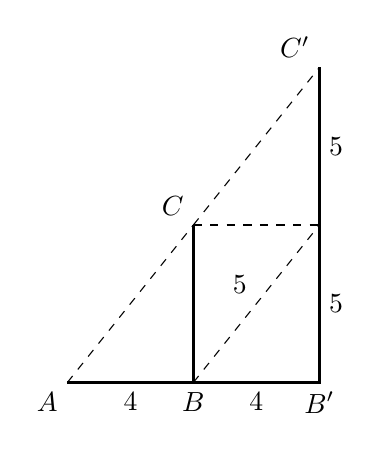
\begin{tikzpicture}
    % constants
    \def\trigwidth{1.6cm}
    \def\trigheight{2cm}
    % small triangle nodes
    \coordinate [label={below left:$A$}]   (A) at (0, 0);
    \coordinate [label={below:$B$}]  (B) at (\trigwidth, 0);
    \coordinate [label={above left:$C$}]  (C) at (\trigwidth, \trigheight);
    % large triangle nodes
    \coordinate [label={below:$B'$}] (B') at (2*\trigwidth, 0);
    \coordinate [label={above left:$C'$}] (C') at (2*\trigwidth, 2*\trigheight);
    \coordinate (B'C'mid) at (2*\trigwidth, \trigheight);
    % lengths labels
    \coordinate [label={below:$4$}] (ABmid) at (0.5*\trigwidth, 0);
    \coordinate [label={below:$4$}] (BB'mid) at (1.5*\trigwidth, 0);
    \coordinate [label={right:$5$}] (x) at (2*\trigwidth, 0.5*\trigheight);
    \coordinate [label={right:$5$}] (y) at (2*\trigwidth, 1.5*\trigheight);
    \coordinate [label={above left:$5$}] (z) at (1.5*\trigwidth, 0.5*\trigheight);
    % small triangle
    \draw [very thick] (A) -- (B) -- (C);
    \draw [dashed] (A) -- (C);
    % large triangle
    \draw [very thick] (B) -- (B') -- (C');
    \draw [dashed] (C) -- (C');
    % internal lines
    \draw [dashed] (C) -- (B'C'mid);
    \draw [dashed] (B) -- (B'C'mid);
\end{tikzpicture}
\caption{Using similar triangles to measure the height of a tree}
\end{figure}

\begin{theorem}
(Thales’ intercept theorem). Consider an arbitrary triangle $ABC$ (see figure \ref{geo:similar-triangles} below) and let $AC$  be extended to $C'$ and $AB$ to $B'$ so that $B'C'$ is parallel to $BC$. Then the lengths of the sides satisfy the relations
\[
\frac{a'}{a} = \frac{b'}{b} = \frac{c'}{c}
\textrm{~ and hence ~}
\frac{a'}{c'} = \frac{a}{c},~~
\frac{c'}{b'} = \frac{c}{b},~~
\frac{b'}{a'} = \frac{b}{a}
\]

\end{theorem}
As these proportions are also preserved when the triangle is displaced and rotated we get the following result. \textit{If corresponding angles of two triangles are equal, then corresponding sides are proportional}. Triangles having these properties are called similar (see \index{similarity}).
\begin{figure}[H]
\label{geo:similar-triangles}
\centering
\begin{tikzpicture}[x=0.6cm,y=0.6cm, rotate=10,every node/.style={draw}]
    % constants
    \def\aLength{3}
    \def\bLength{4}
    \def\cLength{5}
    \def\amLength{6}
    \def\bmLength{8}
    \def\cmLength{10}
    % small triangle nodes
    \coordinate [label={below left:$A$}] (A) at (0, 0);
    \coordinate [label={below:$B$}] (B) at (\cLength, 0);
    \coordinate [label={above left:$C$}] (C) at (\cLength, \aLength);
    % large triangle nodes
    \coordinate [label={below right:$B'$}] (B') at (\cmLength, 0);
    \coordinate [label={above right:$C'$}] (C') at (\cmLength, \amLength);
    % length labels
    \coordinate [label={right:$a$}] (a) at (\cLength, 0.5*\aLength);
    \coordinate [label={above:$b$}] (b) at (0.5*\bLength, 0.5*\aLength);
    \coordinate [label={below:$c$}] (c) at (0.5*\cLength, 0);
    \coordinate [label={right:$a'$}] (a') at (\cmLength, 0.5*\amLength);
    \coordinate [label={above right:$b'$}] (b') at (0.5*\bmLength, 0.5*\amLength+0.75);
    \coordinate [label={below:$c'$}] (c') at (0.5*\cmLength, -0.75);
    % angel labels

    % small triangle
    \draw [very thick] (A) -- (C) -- (B) -- (A);
    % large triangle
    \draw [dashed] (B) -- (B') -- (C') -- (C);
\end{tikzpicture}
\caption{Similar triangles}
\end{figure}

\subsection{Points, Lines and Planes}

\subsection{Angles}

\subsubsection{Radians}
% TODO draw radian drawing
Degrees are often used when introducting geometry. However for more advanced  work we often meassure angles in radians. Radians equals the ratio between the length of an angle arc and its radius. As the circumference of a circle equals $2\pi r$ thus an angle of $360 deg$ equals $\frac{2\pi r}{r} = 2\pi$ radians. Radians allow us to use real numbers in the trigonometric functions, rather than degrees, which are an arbitrary angular measurement between $0-360$. The use of real numbers for meassuring angels allow is essential in more advanced mathematics, calculus for example.

\section{Area and perimeter}
The area of a parallelogram is $a \cdot h$, where h is the altitude of the parallelogram (Eucl. I.35). There are two ways to see this: (a) We cut off the triangle on the left and add it on the right to obtain a rectangle (Euclid’s proof, see the second figure in Fig. 1.11); (b) We cut the parallelogram parallel to AB into a large number of very slim rectangles. The area of a triangle is half the area of the parallelogram.

\subsection{Triangles}
Figure 1.2 shows a right-angled triangle (ie a triangle with one angle of 90°) with another angle denoted by the Greek letter theta θ. The sides of the a right-angled triangle are called the adjacent side (next to θ), the opposite side (opposite to θ) and the hypotenuse (opposite the right-angle).

\subsection{Circle}
\begin{figure}[H]
\begin{tikzpicture}[scale=1.5]
    \tkzDefPoint(0,0){O}
    \tkzDefPoint(1,1){B}
    \tkzDefPoint(0.55,0.45){R}
    \tkzDefPoint(1,0.99){A}
    \tkzDrawArc(O,B)(A)
    \tkzDrawLines[add = 0 and 0](O,A)
    \tkzDrawPoints(O,B)
    \tkzLabelPoints[below](O,R)
    \tkzLabelPoints[right](B)
\end{tikzpicture}
\end{figure}
\noindent The area of a circle is
\begin{equation}
A = \pi \cdot r^2
\end{equation}
the perimeter (circumference) is
\begin{equation}
C = 2\pi \cdot r
\end{equation}

\section{Euclid Elements}
He begins with some definitions of the basic concepts: point, line, circle, triangle, quadrilateral. Euclid then states ten axioms (also called postulates)on which all subsequent reasoning is based. We shall note these merely to see that they do indeed describe apparently unquestionable properties of geometric figures. The first five posgulates are:
\begin{enumerate}
    \item Two points determine a unique straight line
    \item A straight line extends indefinitely far in either direction
    \item A circle may be drawn with any given center and any given radius
    \item All right angles are equal
    \item Given a line l ( Fig. 6–1 ) and a point P not on that line, there exists in the plane of P and l and through P one and only one line m , which does not meet the given line l .
\end{enumerate}

% TODO proof - On a given finite straight line AB to construct an equilateral triangle. A B Γ ∆ E The construction is performed by describing a circle∆centred at A and passing through B (Post. 3) and another circle E centred at B and passing through A (Post. 3). Their point of intersectionΓis then joined to A and to B (Post. 1). The distance AΓis equal to BΓand to AB, which makes the triangle equilateral.

% TODO proof Eucl. I.4, I.8, VI.2 (TODO is this thales theorem)

% TODO proof - The sum of the three angles of an arbitrary triangle ABC is equal to two right angles:

% TODO interestinf geometric things to proof
% - angles of triqngles, quadrilaterals and circles
% - area/of triangles and quadrilaterals 
% - pythagoras (move proof from geometry history book)
% - Squaring the circle. Finding a square whose area is equal to that of a given rectangle
% - Doubling the cube. The problem is:find a cube whose volume is twice that of a given cube
% - Trisecting an angle.
% - Find (all) right-angled triangles with all sides (TODO proof that no more exists)

Adding four right-angled triangles with sides a and b, we arrive at and get the large square of area $(a + b)^2 = a 2 + 2ab + b 2$ . Since the areas of the four triangles add up to $2ab$, the square with area $c^2$ also has area $a^2 + b^2$. 

% TODO proof - An exterior angle of a triangle is greater than either remote interior angle of the triangle.


\section{Classical solid geometry}
\subsection{Cube}
\subsection{Cone}
\subsection{Sphere}

\section{Trigonometry}
% TODO Pythagorean trigonometric identity

\section{Exercises}
\begin{ExerciseList}

% TODO 
% - area calculation excericses (amount of tiles 0.25m^2 tiles needed to cover 15m^2
% - compare area and peremter of squares
% - using thales theorem

\end{ExerciseList}

\chapter{Arithmetic}\label{arit}
% TODO arithmetic missing concepts
% - Ratio (3 to 1 = 3:1 means that for each time there is 3 of one type there is 1 of another).
% -- if a and b are in ratio 5:6 means for each time there is 5 of a there is 6 of b.
% -- if asked how many of type a there are if there are 12 of b we can calculate as (5/6) * 2 = 10/12
% - inequalities http://www.mathsisfun.com/algebra/inequality.html
% - absolute value
% Commutative property of multiplication (changing the order of factors in a multiplication problem and see how it affects the product.)
% Distributive property of multiplication (decomposing the factors in multiplication problems and see how it affects the product.) (9 x 8 = 4x8 + 5x8 = 32 + 40 = 72, 12 * 5 = 6*5 + 6*5 = 30 + 30 = 60)
% Associative property of multiplication (changing the grouping of factors in multiplication problems and see how it affects the product. 2×3×7 = (2×3)×7)
% http://www.theguardian.com/science/alexs-adventures-in-numberland/2015/may/21/how-to-solve-the-maths-puzzle-for-vietnamese-eight-year-olds-that-stumped-parents-and-teachers
% - rates
% \glsentry{cube}{the cube of a number is the number multiplied by itself twice, eg 3 cubed = $3^3 = 3 × 3 × 3 = 27$.}
% \glsentry{integer}{Positive and negative whole numbers such as -34, -5, 0, 1, 17, 1021}
% \glsentry{product}{The result of multiplying together two or more numbers or things, eg the product of 4 and 5 is 20.}
%\glsentry{quotient}{The result of dividing one number by another. The quotient of 14 and 7 is 2 as 14/7 = 2.}

% primes and prime factorization (composite numbers)

% http://www.cs.bu.edu/fac/byers/courses/330/S13/handouts/05multiply.ppt
% http://youtu.be/w4Dy7v-Y5-Y (karetsuba muktiplication)
% https://en.m.wikipedia.org/wiki/Karatsuba_algorithm

% grade school multiplication algorithm 
% - http://www.cim.mcgill.ca/~langer/250/1-gradeschool.pdf
% - http://www.cim.mcgill.ca/~langer/250/2-binary.pdf
% http://jeremykun.com/2014/05/26/learning-to-love-complex-numbers/
% excercise: 2.6598 / 7.8 = 0,341
% 69\4 = 17.25
% TODO define remainder and quotient
% multi digit division and division with decimals

% exponents 
% - http://mathforum.org/library/drmath/view/55603.html 
% - http://primes.utm.edu/glossary/page.php?sort=BinaryExponentiation 

% adding and subtracting in scientific notatio (convert to same base first)

% https://www.khanacademy.org/computing/computer-science/cryptography/modarithmetic/a/the-quotient-remainder-theorem
% https://www.khanacademy.org/computing/computer-science/cryptography/modarithmetic/a/what-is-modular-arithmetic
% https://www.khanacademy.org/computing/computer-science/cryptography/modarithmetic/a/modular-inverses
% http://www.csee.umbc.edu/~stephens/203/PDF/3-4.pdf
% http://mathforum.org/library/drmath/view/52343.html

% shift left (multiply by base n times (in base two a single left shift is the same as multiplying by two)
% shift right (divide by base n times (in base two a single right shift is the same as dividing by two)

% GCD algorithms
% - binary https://en.wikipedia.org/wiki/Greatest_common_divisor#Binary_method
% - https://en.wikipedia.org/wiki/Lehmer%27s_GCD_algorithm
% - http://blog.janmr.com/2009/10/computing-the-greatest-common-divisor.html

% Decimal conversion
% - http://math.stackexchange.com/questions/46864/best-way-of-computing-the-decimal-representation-of-a-fraction-with-an-arbitrary
% - http://mathforum.org/library/drmath/view/63848.html
% - http://programmers.stackexchange.com/questions/192070/what-is-a-efficient-way-to-find-repeating-decimal

% Determine if a number have a finite precision. Repeating decimals in base ten are all fraction with the denominator having at least one prime factors other than two and five  a fraction will terminate if and only if the denominator has for prime divisors only 2 and 5 since every terminating decimal has the form n/10^e, for some e >= 0 as n/10^e = n/(2*5)^e = n/(2^e*5^e)

% Root algorithms
% http://www.mathpath.org/Algor/squareroot/algor.square.root.why.htm
% http://www.mathpath.org/Algor/algor.p-th.root.htm

% Long division algorithm
% http://www.mathpath.org/Algor/algor.long.div.htm
% - binary https://www.quora.com/How-do-I-divide-two-numbers-using-only-bit-operations-in-Java
% - http://mathlesstraveled.com/2008/09/07/rational-numbers-and-decimal-expansions/

% Integer square root
% - http://www.embedded.com/electronics-blogs/programmer-s-toolbox/4219659/Integer-Square-Roots
% - http://stackoverflow.com/a/30136377

% floor and ceiling http://blog.janmr.com/2009/09/useful-properties-of-the-floor-and-ceil-functions.html
% http://math.stackexchange.com/a/344818
% http://math.stackexchange.com/questions/1202456/how-to-calculate-the-integer-portion-of-a-fraction-using-only-div-and
% http://math.stackexchange.com/a/582983
% truncate (same as integer part http://planetmath.org/integerpart)  For positive numbers, trunc and floor give the same result. But for negative numbers, floor rounds down and trunc rounds up. This is because trunc always rounds toward 0.
% IntegerPart[x]+FractionalPart[x] is always exactly x.

% Fibonachi
% - http://blog.janmr.com/2011/03/evaluation-of-fibonacci-numbers.html

% Powers
% - http://blog.janmr.com/2011/01/evaluation-of-powers.html

% arithmetic 
% - http://blog.janmr.com/2011/10/multiple-precision-addition.html
% - http://blog.janmr.com/2011/10/multiple-precision-subtraction.html
% - http://blog.janmr.com/2011/11/basic-multiple-precision-multiplication.html
% - http://blog.janmr.com/2012/11/basic-multiple-precision-short-division.html




Numbers are an integral part of nature; a day can be split into $24$ equal parts, each of our hands has five fingers and so on. Thus even without any formal study of arithmetic humans have a basic understanding of numbers

\myindent The earliest known formal concepts of numbers dates back to the Babylonian, Egyptian and later Greek and Roman civilizations. Here tax collectors used tables to record tax payments and in the process came up with various standardised shorthands to record their work. For example if a citizen payed five animals a tax collector may have written \rom{1}\rom{1}\rom{1}\rom{1}\rom{1}. Each \rom{1} representing one animal. If later additional five animals where collected he may have recorded \rom{10} instead of \rom{1}\rom{1}\rom{1}\rom{1}\rom{1}\rom{1}\rom{1}\rom{1}\rom{1}\rom{1} as its easer to read. From these early shorthands rose the first numerical systems where it was agreed to let specific symbols represent a quantity. By far the most successful of these was the, still familiar, roman symbols \rom{1}, \rom{2}, \rom{3}, \rom{4}, \rom{5}, \rom{6}, \rom{7}, \rom{8}, \rom{9} and \rom{10}. 

\myindent Once number systems where established their properties was explored. The \rom{7} book of Euclid's elements published around 300 BC. deals extensively with elementary number theory including divisibility and the existence of \index{prime}{prime numbers}. The concept of rational (fractional) numbers was introduced early as a useful device for division, such as dividing the land belonging to a village among its inhabitants for harvesting. Egyptians used the word "nfr" to denote zero balance in accounting and later during the $7th$ century AD, negative numbers were used in India to represent debts.

\myindent The use of numbers in trading and science quickly outgrew the capabilities of early numerical systems. The romans for example had no concept of position where the same symbol is reused in different positions to denote different values. Thus they continuously had to invent new symbols for new numbers such as \rom{100} for $100$ and \rom{1000} for $1000$. As the system grew more complex it resulted in cryptic quantities such as \rom{11111} for $11111$. These shortcomings eventually led to the creation of simpler and better systems. Around $400 AD$ a new positional system began surfacing in India based on the now familiar ten numbers $0-9$. 

\section{Hindu numeral system}
The Hindu numeral system was invented between the $1st$ and $4th$ century and then later adopted by Persian and Arab mathematicians in the $9th$ century. From the $14th$ century Roman numerals gradually began to be replaced by it. The main advantage of the Hindu system is that it greatly simplifies operations such as addition and subtraction. Also its use of position to denote order of magnitude ensures it requires far fewer different symbols to represents numbers. For example the number $2506$ really represents
\[
2506 = 2 \times 1000 + 5 \times 100 + 0 \times 10 + 6 \times 1
\]
and the number $203$ is represented as 
\[
213 = 2 \times 100 + 1 \times 10 + 3 \times 1
\]
to add these we simply add the numbers in each position
\begin{align*}
2506 + 213 =& 2 \times 1000 + (5+2) \times 100 + (0+1) \times 10 + (6+3) \times 1 \\
           =& 2 \times 1000 + 7 \times 100 + 1 \times 10 + 9 \times 1 \\
           =& 2719 
\end{align*}
or more familiarly 
\begin{figure}[H]
\centering
\opadd{2506}{213}
\end{figure}

Using the exponent notation 
\[
10^{n} = \underbrace{10 \times \dots \times 10}_{n}
\]
that is $10^1 = 10$, $10^2 = 10 \times 10 = 100$ and $10^3 = 10 \times 10 \times 10 = 1000$ and taking advantage of that $10^0 = 1$ we can rewrite $2506$ as
\[
2506 = 2 \times 10^{3} + 5 \times 10^{2} + 0 \times 10^{1} + 6 \times 10^{0}.
\]
and in general we can write any possible integer $a_{n}a_{n-1} \cdots a_{1}a_{0}$ as
\begin{equation}\label{arit:int-system}
a_{n}a_{n-1} \cdots a_{1}a_{0} = a_{n} \times 10^{n} + a_{n-1} \times 10^{n-1} + \cdots + a_{1} \times 10^{1} + a_{0} \times 10^{0} 
\end{equation}
where each digit $a$ is a number between $0$ and $9$ and a sequence like $a_{3}a_{2}a_{1}a_{0}$ represents a four digit number such as $2506$. Using the \index{Sigma notation}{sigma notation} as a shorthand for sums 
\[
\sum_{k=1}^{n} k = \underbrace{1 + \dots + n}_{n}
\]
that is the sum $1 + 2 + 3 + 4 + 5 + 6$ can be written as 
\[
\sum_{n=1}^{6} n 
\]
and the sum $10^0 + 10^1 + 10^2 + 10^3$ can be written as
\[
\sum_{n=0}^{3} 10^n
\]
we can simplify \ref{arit:int-system} to
\begin{equation}
a_{n}a_{n-1} \cdots a_{1}a_{0} = \sum_{k=0}^{n} a_{k}10^{k}
\end{equation}

\section{Fractions and decimal numbers}
% TODO
% [Simplifying Fractions] (TODO examples 78/52
% [Converting fractions to decimals]

The concept of fractions predates the hindu numerals as way of dividing a whole into parts. For example a farmer may decide to split his land into $4$ parts storing the crops from the three parts and selling the crops from the remaining one part. Thus the fraction $\frac{3}{4}$ represents the crops to keep and the remaining $\frac{1}{4}$ those to sell and $\frac{4}{4}$ represents the entire land. In the fraction $\frac{3}{4}$ the number $3$ is known as the \index{Numerator}{numerator} and tells us that the fraction represents $3$ equal parts. The \index{Denominator}{denominator} $4$ tells us that $4$ parts make up a whole. Equally the fraction $5/4$ tells us that $4/4$ makes up a whole and we have an extra $1/4$ part left. As fractions represents equal parts we need to take care when performing arithmetic on them. Consider the meaning of splitting two equal size pizzas such that one is cut into $3$ parts and the other into $4$ parts. Clearly $3/3 = 4/4$ since getting all of the slices of either pizza would equal to getting the entire pizza. However one slice of the pizza cut into three pieces is greater than one from the pizza cut into four, so that $1/3 > 1/4$. Thus when comparing the size of fractions we need to take into account how many equal parts makes up whole and how many of those we have. In general we have
\begin{equation}
\frac{a}{b} < \frac{c}{d} \text{if and only if $ad < bc$}.
\end{equation}
so when comparing $3/4$ to $5/7$ we compute $3 \times 7 = 21$ and $5 \times 4 = 20$ and as $21 > 20$ we know that $3/4 > 5/7$. From this we also see that two fractions have the same value when they represent the same parts of a hole e.g. 
\begin{equation}
\frac{a}{b} = \frac{c}{d} \text{if and only if $a \times d = b \times c$}.
\end{equation}
Its interesting to note that a fraction preservers its value when we multiply the numerator and denominator with the same value that is 
\[
\frac{1}{2} = \frac{2 \times 1}{2 \times 2} = \frac{2}{4} 
\]
the rational from this being that getting one part of a pizza cut into halves results in the same amount of pizza as if receiving two slices of the same pizza cut into four parts. When adding or subtracting fractions we need to be extra vigilant. Adding $1/3$ to $1/4$ does not yield $2/7$. Instead we can only add or subtract two fractions when they represents the same division of a whole, that is they have a common denominator.
In this case we can multiply the numerator and denominator of $1/4$ with $3$ to obtain the common denominator $12$ observing that this new fraction has the same value as the old as 
\[
\frac{1}{4} = \frac{3 \times 1}{3 \times 4} = \frac{3}{12}
\]
Seminally we can multiply the numerator and denominator of $1/3$ with $4$ to obtain the same denominator i.e 
\[
\frac{1}{4} = \frac{4 \times 1}{4 \times 3} = \frac{4}{12}
\] 
and now we can add the two numbers as 
\[
\frac{1}{3} + \frac{1}{4} = \frac{4}{12} + \frac{3}{12} = 7/12
\] 
In general when adding fractions
\begin{equation}
\frac{a}{b} + \frac{c}{d} = \frac{a \times d + b \times b}{b \times d}
\end{equation}
and when subtracting them 
\begin{equation}
\frac{a}{b} - \frac{c}{d} = \frac{a \times d - c \times b}{b \times d}
\end{equation}
Here we make good use of a simple way of obtaining a common denominator by multiplying each fraction by the denominator of the other. 

% TODO describe decimals here
Place the decimal in the numerator and one in the denominator and multiply both with multiples of ten until the decimal point disapears e.g. $0.024 = 0.024/1 = 0.24/10 = 2.4/100 = 24/1000$

\begin{description}
\item [Multiplying fractions] $\frac{a}{b} * \frac{c}{d} = \frac{a*b}{c*d}$
\item [Dividing fractions] Division is equivalent to multiplying by the
reciprocal of the divisor fraction: $\frac{a}{b}/\frac{c}{d} =
\frac{a}{b} \cdot \frac{d}{c}$
\end{description}

\subsection{Mixed numbers}
Improper fractions such as $5/4$, where the numerator is larger than the denominator, are commonly represented as a combination of a whole number and a proper fraction called a mixed number e.g. $5/4 = 1\frac{1}{4}$.
\begin{description}
\item [Converting fractions to mixed numbers] Convert the numerator to a sum where the first part can be divided by the denominator and the last part has a lower value than the denominator e.g. $\frac{64}{5} = \frac{60 + 4}{5} = \frac{60}{5} + \frac{4}{5} = 12 \frac{4}{5}$
\item [Converting mixed numbers to fractions] Multiply the leading integer with the denominator and add it to the numerator e.g. $12 \frac{2}{3} = \frac{3 * 12 + 2}{3} = \frac{38}{3}$
\item [Adding and subtracting mixed numbers] A mixed number $a \frac{b}{c}$ is a short hand for $a + \frac{b}{c}$ so to add or subtract mixed numbers perform the operation step wise on the integer and fractional part of the numbers e.g. $6\frac{6}{12} - 3\frac{3}{5} = 6 + \frac{6}{12} - 3 - \frac{3}{5} = 2\frac{9}{10}$.
\item [Multiplying mixed numbers] Convert the mixed number to a fraction and multiply these e.g. $1\frac{1}{4} * 4 = \frac{20}{4} = 5$
\end{description}


The system is easily extended to handle decimal numbers such as $2506.12$. If we use the exponent notation
\[
10^{-n} = \frac{1}{10^{n}}
\]
that is $10^{-1} = \frac{1}{10} = 0.1$ and $10^{-2} = \frac{1}{100} = 0.01$. We can rewrite $2506.12$ as 
\begin{align*}
2506.12 =& 2 \times 1000 + 5 \times 100 + 0 \times 10 + 6 \times 1 + 1 \times 0.1 + 2 \times 0.01 \\
        =& 2 \times 10^{3} + 5 \times 10^{2} + 0 \times 10^{1} + 6 \times 10^{0} + 1 \times 10^{-1} + 2 \times 10^{-2} 
\end{align*}
Generally we represent a number with $n$ integer digits $a_{n}a_{n-1} \cdots a_{1}a_{0}$ and $m$ decimal digits 
$b_{1}b_{2} \cdots b_{m-1}b_{m}$ as 
\begin{equation}\label{arit:decimal-system}
a_{n}a_{n-1} \cdots a_{1}a_{0}.b_{1}b_{2} \cdots b_{m-1}b_{m} = \sum_{k=0}^{n} a_{k}10^{k}.\sum_{k=1}^{m} b_{k}10^{-k}
\end{equation}
From the above formula we also see why when a decimal number is multiplied by $10$, every figure moves one place to the left
\begin{align*}
1.25 \times 10 =& (1 \times 10^0 + 2 \times 10^{-1} + 5 \times 10^{-2}) \times 10 \\
               =& 1 \times 10^1 + 2 \times 10^0 + 5 \times 10^{-1} \\
               =& 12.5 
\end{align*}
and when divided by $10$, every figure moves one place to the right 
\begin{align*}
\frac{1.25}{10} =& 1.25 \times 10^{-1} \\
                =& (1 \times 10^0 + 2 \times 10^{-1} + 5 \times 10^{-2}) \times 10^{-1} \\
                =& 1 \times 10^{-1} + 2 \times 10^{-2} + 5 \times 10^{-3} \\
                =& 0.125 
\end{align*}

\section{Basic properties of numbers}
One of the many advantages of the positional number system is how it makes comparison of numerical values easy. In the roman numeral system this was only possible by memorising the quantities represented by each symbol; one simply had to remember that \rom{1000} was larger than \rom{100}. In the positional system we only need to compare the value of each digit in each position. To make this easy names for each position has been invented, some of these are listed below
\begin{figure}[H]
\centering
\begin{tabular}{|l|l|l|l|}
\hline
\textbf{Decimal name} & \textbf{Decimal position}  \\ \hline
thousands	         & $10^3 = 1000$               \\ \hline
hundreds	             & $10^2 = 100$                \\ \hline
tens	                 & $10^1 = 10$                 \\ \hline
ones	                 & $10^0 = 1$                  \\ \hline
tenths	             & $10^{-1} = 0.1$             \\ \hline
hundredths	        & $10^{-2} = 0.01$             \\ \hline
thousandths	        & $10^{-3} = 0.001$           \\ \hline
\end{tabular}
\end{figure}
To compare $1000$ to $999$ we simply begin from the highest digit and work our way down. Since the first number has $1$ in the thousands place and the second has a zero ($999= 0999$) we know that $1000$ is greater than $999$ and we write $1000>999$. Generally if one number $a$ is larger than another $b$ we write $a > b$ and if smaller we write $b < a$. If all the digits are the same then the numbers are equal and we write $a=b$. 

\myindent Sometimes, for example when comparing the speed of cars, we are only interested in how far one number is from another. If the speed limit is $100$ and you are going $70$ and another driver is going $130$, both of you will likely get a ticket. This is because the difference between you and everybody else is $30$. Not $-30$ and $30$ but $30$. This concept is called \index{absolute value}{absolute value}. The absolute value of a integer $x$ is written $\abs{x}$ and is simply the numerical value obtained by removing any negative sign. Formally we write
\begin{equation}
  \abs{x}=\begin{cases}
    x, & \text{if $x \geq 0$.}\\
   -x, & \text{if $x < 0$.}
  \end{cases}
\end{equation}
So the absolute value of $\abs{-30} = 30$ and that of $\abs{30} = 30$. 

\myindent In many cases its only necessary to compare numbers to a certain precision for example when comparing the population of one country to another we may be satisfied to count their populations in millions. This is the process of \index{Rounding}{rounding}. The idea is to replace a number by another approximately equal value that has a shorter or simpler representation. The procedure is as follows: \textit{Pick the number to round to as the last digit to keep, leave it the same if the next digit is less than $5$ or increase it by $1$ if the next digit is $5$ or more. Finally turn all following digets into zeros}. The basic algorithm is as follows
\begin{algorithm}[H]
    \caption{Rounding algorithm}
    \label{arit:rounding}
    \begin{algorithmic}[1]
        \Procedure{Round}{$n,i$} \Comment{Round $n$ to $i$'th place}
            \State $digits \gets digitsOf(n)$ \Comment{Array with digits of $n$}
            \State $inc \gets 0$
            \If{$digits[i-1] > 4$}           \Comment{Increase digit if above $4$}
                 \State $inc \gets 10^{i}$  
            \EndIf
            \While{$i > 0$}                    \Comment{Zero out remaining digits}
               \State $digits[i-1] = 0$      
               \State $i \gets i - 1$
            \EndWhile
            \State $r \gets numberOf(digits) $ \Comment{Turn array into number}
            \State $r \gets r + inc$     
            \State \textbf{return} $r$  \Comment{The rounded value of $n$}
        \EndProcedure
    \end{algorithmic}
\end{algorithm}
If we want to round the number $1997$ to the nearest ten ($i$ becomes $1$ as $10^1 = 10$) we first turn it into an array $\left[1,9,9,7\right]$ then examine the digit in the $i-1$ position which is $7$. As this is above $4$ we determine to increment the number by $10$. The lower digits are then zeroed out to $\left[1,9,9,0\right]$ and turned into the number $1990$ which we add the $10$ to form the final result $2000$. Besides the standard rounding method mentioned above two other popular methods exists called \index{Floor}{floor} and \index{Ceiling}{ceiling}. These maps a decimal number to the largest previous or the smallest following integer, respectively. More precisely, $floor(x) = \lfloor x \rfloor$ is the largest integer not greater than $x$ and $ceiling(x) =  \lceil x \rceil$ is the smallest integer not less than $x$. The following table should clarify how their difference
\begin{figure}[H]
\centering
\begin{tabular}{|l|l|l|l|}
\hline
\textbf{Value}  & \textbf{Floor} & \textbf{Ceiling} & \textbf{Fractional part} \\ \hline
2.4	            & 2	            & 3	              & 0.4                      \\ \hline
2.9	            & 2	            & 3	              & 0.9                      \\ \hline
-2.7	            & -3	            & -2	              & 0.3                      \\ \hline
-2	            & -2	            & -2	              & 0                        \\ \hline
\end{tabular}
\end{figure}

Another device for easily comparing and writing numbers was invented when scientist began studying very large and small quantities. Using ordinary decimal numbers became inconvenient. To remedy this \index{Scientific notation}{scientific notation} was invented in which all numbers are written in the form
\[
a \times 10^b
\]
where the exponent $b$ is chosen so its absolute value is at least one but less than ten ($1 \leq |a| < 10$). Thus $350$ is written as $3.5×10^2$. Sometimes the so called \textit{E notation} is used where we write $e$ in the exponent instead of $10$ that is
\[
3.0 \times 10^{-9} = 3.0e−9
\]
this notation was originally invented as calculators could not display exponents correctly. Note that the $E$ or $e$ should not be confused with Euler's number $e$ which holds a completely different significance. The following table are examples of scientific notation:
\begin{figure}[H]
\centering
\begin{tabular}{|l|l|l|l|}
\hline
\textbf{Decimal notation}   & \textbf{Scientific notation} \\ \hline
2                           & $2 \times 10^0$              \\ \hline
300                         & $3 \times 10^2$              \\ \hline
4,321.768                   & $4,321768 \times 10^3$       \\ \hline
−53,000                     & $−5,3 \times 10^4$           \\ \hline
6,720.000.000	           & $6,72 \times 10^9$           \\ \hline
0.2	                        & $2 \times 10^{−1}$           \\ \hline
0,000.000.007.51	           & $7,51 \times 10^{−9}$        \\ \hline
\end{tabular}
\end{figure}
This form allows easy comparison of numbers, as the exponent $b$ gives the number's \index{order of magnitude}{order of magnitude}. For example, the order of magnitude of $1500$ is $3$, since $1500$ is written as $1.5 × 10^3$. When adding and subtracting two numbers in scientific notation, we must adjust the two values so that their exponents are the same. For example, when adding $1.23e1$ and $4.56e0$, we first adjust $4.56e0$ to $0.456e1$ and then add it to $1.23e1$ which produces $1.686e1$.

\section{Arithmetic in the Hindu numeral system}
As mentioned the perhaps biggest advantage of the Hindu numeral system was the ease with which merchants and scientist could carry out calculations such as addition, subtraction, multiplication and division

The order of arithmetic operators is as follows
\begin{enumerate}
\item Parentheses and exponents
\item Multiplication and division
\item Addition and subtraction
\end{enumerate}
When multiple operations exists on the same level you do the one that it closest on the left, for example
\[
2-10+8-(-2)+(-10) = 2 - 10 + 8 + 2 - 10 
= (2 - 10 + 8) + 2 - 10 = (-8 + 8) + 2 - 10 = 0 + 2 - 10 = -8
\]


\subsection{Addition}
% TODO missing addition concepts
% - describe adding decimals
Addition represents the operation of adding objects to a collection. For example, $2+3$ can be though of as if you have $2$ apples and someone give you $3$ more, then you have $5$ apples in total. Assuming $b$ is positive then on a number line $a+b$ represents starting on number $a$ and moving $b$ places to the right. Similar if $b$ is negative then $a+b$ represents starting on number $a$ and moving $b$ places to the left. Unlike subtraction the addition operations is both commutative (that is $a + b = b + a$) and associative (that is $a + (b + c) = (a + b) + c$)

\begin{description}
\item [Adding integers] We add integers by adding the ones, tens,hundreds etc. in each number individually, starting from the right. If the result of addition is above $10$ then we subtract $10$ from the result and add one (known as a carry) to the next group to be added. For example
\begin{figure}[H]
\centering
\opadd{143}{89}
\end{figure}
That is we add $3+9=12$ as the result is above $10$ we subtract $10$ from it and add one tenth to the tenths place. In the tenth place we now add $1+3+8=12$ which again is above $10$, so we subtract $10$ from it and add $1$ to the hundreds place (ten tens being one hundred) and so finally we add $1+1$ in the hundreds place.

To understand why this procedure works consider that the number $143 = 100 + 40 + 3$ and $89 = 80 + 9$ so we can do
\[
\begin{align}
143 + 89 &= (100 + 40 + 3) + (80 + 9) \\
         &= 100 + (40+80) + (3+9)     \\
         &= 100 + 120 + 12            \\
         &= 232
\end{align}
\]
\item [Adding decimals] We add decimals similar to integers by starting
from the rightmost decimal.
\begin{figure}[H]
\centering
\opadd{9.087}{15.924}
\end{figure}
\end{description}

\begin{algorithm}[H]
    \caption{Add two N digit numbers a and b represented as arrays of digits}
    \label{arit:addition}
    \begin{algorithmic}[1]
        \Procedure{Addition}{$a,a$} 
            \State $carry \gets 0$ 
            \For{$i=0 \text{ to } N-1$} 
                \State $sum \gets a[i] + b[i] + carry$
                \State $carry \gets sum / 10$ \Comment{TODO}
                \State $r[i] \gets sum \% 10$ \Comment{TODO}
            \EndFor
            \State $r[N] \gets carry$
            \Return $r$  
        \EndProcedure
    \end{algorithmic}
\end{algorithm}
% TODO explain div and mod                 \State $carry \gets (a[i] + b[i] + carry)/10$
% r[i] \gets (a[i] + b[i] + carry) % 10

\subsection{Subtraction}
Subtraction represents the operation of removing objects from a collection. For example, $5-2$ can be though of as if you have $5$ apples and take $2$ away, then you have $3$ apples left. Assuming $b$ is positive then on a number line $a-b$ represents starting on number $a$ and moving $b$ places to the left. Similar if $b$ is negative then $a-b$ represents starting on number $a$ and moving $b$ places to the right.

Subtraction is not commutative, that is $a - b \neq b - a$ instead we can reverse the subtraction order by $a - b = -(b - a) = -b + a$. Further subtraction is not associative so $a  - (b - c) \neq (a - b) - c$ instead it holds $a - b - c = a - (b + c)$ and $a - b - c - d = a - (b + c + d)$ and so on.
\begin{description}
\item [Subtracting integers] We subtract numbers by subtracting each
ones, tens, hundreds etc. individually, starting from the right, if the
subtraction yields a result less than zero then we borrow ten from the
number to the left by decreasing its value by one:
\begin{figure}[H]
\centering
\opsub{133}{89}
\end{figure}
\item [Subtracting decimals]
% TODO subtracting decimals
\end{description}

\subsection{Multiplication}
Multiplication of two whole numbers is equivalent to the addition of one of them with itself as many times as the value of the other one; for example, $3 \cdot 4$ can be calculated by adding $4$ to itself $3$ times:
\[
3 \cdot 4 = 4 + 4 + 4 = 12
\]
it can also be calculated by adding $4$ copies of $3$ together:
\[
3 \cdot 4 = 3 + 3 + 3 + 3 = 12
\]
Formally we say that multiplication is both commutative (i.e. the order in which two numbers are multiplied does not matter $a \cdot b = b \cdot a$) and associative $a \cdot (b \cdot c) = (a \cdot b) \cdot c$. Multiplication has other important properties:
\begin{description}
\item [Distributive property] Holds with respect to multiplication over addition. This identity is of prime importance in simplifying algebraic expressions: $x\cdot(y + z) = x\cdot y + x\cdot z$
\item [Identity element] The multiplicative identity is $1$; anything multiplied by one is itself. This is known as the identity property: $x\cdot 1 = x$
\item [Zero element] Any number multiplied by zero is zero. This is known as the zero property of multiplication: $x\cdot  0 = 0$
\end{description}

% TODO missing multiplication areas
% - factors and products
% - explain operations of single and multi diget
% - explain meaning of multiplying negative numbers
% - explain techniques for muktiplication
\begin{description}
\item [Multiplying integers] We multiply integers by multiplying the ones, tens, hundreds etc. in each number individually, starting from the right. If the result of multiplication is above $10$ we subtract $10$ from the result and add one (known as a carry) to the next group to be multiplied. For example
\begin{figure}[H]
\centering
\opmul[displayintermediary=None]{142}{3}
\end{figure}

That is we first multiply $3 \cdot 2 = 6$ in the ones place, then in the tenth place we multiply $3 \cdot 4 = 12$ which is above $10$, so we subtract $10$ from it and add $1$ to the hundreds place and so finally we multiply $3 \cdot 1 = 3$ and add the carry of $1$ to it in order to get $4$ in the hundreds place.

To understand why this procedure works consider that the number $142 = 100 + 40 + 2$ so really we have
\[
\begin{align}
143 \cdot 3 &= (100 + 40 + 2) \cdot 3  \\
            &= (100 \cdot 3) + (40 \cdot 3) + (2 \cdot 3)  \\
            &= (100 \cdot 3) + (10 \cdot 4 \cdot 3) + 6  \\
            &= (100 \cdot 3) + (10 \cdot 12) + 6  \\
            &= (100 \cdot 3) + (100 + 20) + 6  \\
            &= (100 \cdot 4) + 20 + 6  \\
            &= 426
\end{align}
\]

\item [Multiplying decimals] To multiply decimals convert them into integers, multiply them and then convert the result back to a decimal i.e.
\begin{itemize}
\item $8 * 0.8 = 8 * \frac{8}{10} = \frac{64}{10} = 6.4$
\item $2.91 * 3.2 = \frac{291}{100} * \frac{32}{10} = \frac{291 * 32}{1000} =
\frac{9312}{1000} = 9.312$
\end{itemize}
\end{description}

When multiplying numbers of different precision care should be taken when deciding on the preccion of the result. To facilitate this the concept of \index{significant figures}{significant figures} has been invented. The significant figures of a number are those digits that carry meaning contributing to its precision. The procedure for identifying significant figures is as follows 
\begin{enumerate}
\item Identify the non-zero digits and any zeros between them. These are all significant.
\item Leading zeros are not significant.
\item If its a decimal, then trailing zeros are significant.
\end{enumerate}
for example
\[
1.234 \times 2.0 = 2.468\cdots \equiv 2.5
\]
here the first factor $1.234$ has four significant figures and the second $2.0$ has two significant figures. The factor with the least number of significant figures is the second one with only two, so the final result should also have a total of two significant figures.




\subsection{Division}
% TODO missing division
% - using  prime factorisation to simplify numbers (see number theory)
% - factors
% - GCD and LCM
% - explain why division algo works
% - division commutativity and associative
\begin{description}
\item [Dividing improper fractions] Division is really counting the number of repeated subtractions of the divisor into the dividend e.g. $3024/42 = 72$ as shown below
\newline
\[
\begin{array}{*{6}{>{\hfill}m{7mm}}}
 &
     &
         0&
             0&
                 7&
                     2\\\cline{3-6}
4&
  2\big)&
        3&
             0&
                 2&
                     4\\\cline{1-2}
 &
     &
        2&
            9&
                4&
                     \\\cline{3-5}
 &
     &
         &
             &
                8&
                     4\\
 &
     &
         &
             &
                 8&
                     4\\\cline{5-6}
\end{array}
\]
\item [Dividing proper fractions] As proper fractions always represent values parts less than 1 whole we know the result must be a decimal beginning with 0.
\[
\begin{array}{*{7}{>{\hfill}m{7mm}}}
 &
     &
         &
           0,&
                7&
                    0&
                        3\\\cline{3-7}
2&
  7\big)&
        1&
           9,&
                0&
                    0&
                        0\\\cline{1-2}
 &
     &
        1&
            8&
                9&
                     &
                         \\\cline{3-5}
 &
     &
         &
             &
                1&
                    0&
                        \\
 &
     &
         &
             &
                 &
                     0&
                        \\\cline{5-7}
 &
     &
         &
             &
                 1&
                     0&
                         0\\
 &
     &
         &
             &
                 &
                     8&
                         1\\\cline{6-7}
 &
     &
         &
             &
                 &
                     1&
                         9\\
\end{array}
\]
\item [Dividing decimals] To divide decimals first convert the denominator into a integer then divide the resulting fraction as shown above e.g. $3.3534/0.81 = 335.34/81$
\[
\begin{array}{*{7}{>{\hfill}m{7mm}}}
 &
     &
        0&
            0&
                4,&
                    1&
                        4\\\cline{3-7}
8&
  1\big)&
        3&
            3&
                5,&
                    3&
                        4\\\cline{1-2}
 &
     &
        3&
            2&
                4&
                     &
                         \\\cline{3-5}
 &
     &
         &
             1&
                1&
                    3&
                        \\
 &
     &
         &
             &
                 8&
                     1&
                        \\\cline{5-7}
 &
     &
         &
             &
                 3&
                     2&
                         4\\
 &
     &
         &
             &
                 3&
                     2&
                         4\\\cline{6-7}
\end{array}
\]

\end{description}

\subsection{Divisibility tests}
% TODO proove these
The following rules can test numbers for divisibility
\begin{description}
\item [Divisible by $2$] if the last didget is divisible by $2$.
\item [Divisible by $3$] if the sum of the digits is divisible by $3$.
\item [Divisible by $4$] if the number formed by the last two digits is
divisible by $4$.
\item [Divisible by $5$] if the last digit is either $0$ or $5$.
\item [Divisible by $6$] if divisible by $2$ and $3$.
\item [Divisible by $9$] if the sum of the digits is divisible by $9$.
\item [Divisible by $10$] if the last digit is $0$.
\end{description}

\subsection{Remainder}
The remainder from the division $a/b$ is represented mathematically as $a \textrm{mod} b$, for example $9/2 = 4$ and $9 mod 2 = 1$. In general to the find the result of $a \textrm{mod} b$ we follow these steps:
\begin{enumerate}
\item Construct a clock with size $b$
\item Start at 0 and move around the clock $a$ steps (If the number is positive we step clockwise, if it's negative we step counter-clockwise).
\item Wherever we land is our solution.
\end{enumerate}
For example $7 mod 2 = 1$ since we can make a clock with numbers $0,1$ then start at $0$ and go through $7$ numbers in a clockwise sequence $1,0,1,0,1,0,1$. Similar $-5 mod 3 = 1$ since we make a clock with numbers $0,1,2$ then start at $0$ and go through $5$ numbers in counter-clockwise sequence  $2,1,0,2,1$




this let to the general rule that
\[
x^m \times x^n = x^{m+n}
\]
Similarly, dividing exponents $\frac{x^3}{x^2} = \frac{x \times x \times x}{x \times x} = x = x^1 = x^{3-2}$ let to the generalisation that 
\[
\frac{x^m}{x^n} = x^{m-n}
\]
Early in the development of exponent notation the above rule encountered issues when the exponent of the denominator was greater than that of the numerator, as in $x^3/x^5$, where the rule would give us $x^{3-5} = x^{-2}$. However by letting $x^{-n} = 1/x^n$ we obtain $x^{3-5} = x^{-2} = 1/x^2$ which agrees with the results of dividing $x^3$ by $x^5$ directly. When $m = n$ the above rule leads $x^m/x^n = x^{m-n} = x^0$ which we must define as one. 

\section{Exponents and logarithms}\label{arit:exp}
If we multiply 3 by itself 4 times we get
\[
3 \cdot 3 \cdot 3 \cdot 3 = 81
\]
A more concise way of writing this is to say
\[
3^4 = 81
\]
where 3 is the base and the superscript 4 is called the power or exponent.

% TODO compare list of rules with that from math picture taken

\begin{description}
\item [Squares $b^2$] means $b \cdot b$ and is read \emph{b squared} because $b^2$ is the area of a square whose side has length $b$.
\item [Cubes $b^3$] means $b \cdot b \cdot b$ and is read \emph{b cube} because $b^3$ is the volume of a cube whose side has length $b$.
\item [Powers of $10$] If the power is positive the result is one followed by as many zeros as the number in the exponent $10^7 = 10000000$. If the exponent is negative we have as many zeroes as the exponent followed by one with the first zero being before the comma the rest after $10^+7 = 0.0000001$
\item [Negative powers] $a^{-n} = \frac{1}{a^n}$
\item [Products of powers] $a^n \cdot a^m = a^{n+m}$ this can be seen as $5^3 \cdot 5^2 = (5 \cdot 5 \cdot 5) \cdot (5 \cdot 5)= 5^5$
\item [Products of unlike powers] $a^n \cdot b^n = (a \cdot b)^n$ this can be seen as $(2 \cdot 2 \cdot 2) \cdot (3 \cdot 3 \cdot 3) = (2 \cdot 3) \cdot (2 \cdot 3) \cdot (2 \cdot 3) = (2 \cdot 3)^3$
\item [Fractions of powers] $\frac{a^n}{a^m} = a^{n-m}$ this can be seen as $\frac{5^3}{5^2} = \frac{5 \cdot 5 \cdot 5}{5 \cdot 5} = 5^1$
\item [Powers of fractions] $\left(\frac{a}{b}\right)^n = \frac{a^n}{b^n}$ this can be seen as $\left(\frac{2}{3}\right)^3 = \frac{2}{3} \cdot \frac{2}{3} \cdot \frac{2}{3} = \frac{2^3}{3^3}$
\item [Powers of powers] $(a^m)^n = a^{(m \cdot n)}$ this can be seen as $(5^2)^3 = 5^2 \cdot 5^2 \cdot 5^2 = 5^{6}$
\item [Fractional powers] $a^{\frac{x}{y}} = (a^{\frac{1}{y}})^x$. This can be related to roots since $\sqrt{a} \cdot \sqrt{a} = a$ can be satisfied as $a^{x} \cdot a^{x} = a^{x+x} = a^{1}$ only when $x = 1/2$. That is $\sqrt{a} = a^{1/2}$. Generally we have $\sqrt[n]{a} = a^{1/n}$.
\item [Simplifying radicals] Radicals such as $\sqrt{32}$ are simplified by rewriting them to lower terms using the above rules e.g. $3\sqrt{8} - 6\sqrt{32} = 3\sqrt{4}\sqrt{2} - 6\sqrt{16}\sqrt{2} = 6\sqrt{2} - 24\sqrt{2} = -18\sqrt{2}$. Often it can be constructive to rewrite radicals using their prime factorisation e.g. $\sqrt[3]{81} = \sqrt[3]{9 \cdot 9} = \sqrt[3]{3 \cdot 3 \cdot 3 \cdot 3} = 3\sqrt[3]{3}$
\item [Exponentiation of fractions] If $n$ is a non-negative integer, then
$\left(\frac{a}{b}\right)^{n} = \frac{a^n}{b^n}$ and if $a \neq 0$ then
$\left(\frac{a}{b}\right)^{-n} = \frac{1}{\left(\frac{a}{b}\right)^n} =
\frac{1}{\frac{a^n}{b^n}} =\frac{b^n}{a^n}$.
\end{description}

The use of exponents was greatly boosted by the Scottish landowner {John Napier}\index{John Napier} (1550-1617) who invented {logarithms}\index{logarithms} while searching for a way to simplify computation of large numbers. His idea was to utulize the $x^n \times x^m = x^{n+m}$ property of exponents to simplify multiplication and division as it was generally agreed that multiplication and devision was more difficult than addition and subtraction. 

His line of thought was this: If we could write any positive number as a power of some given, fixed number (later to be called a base), then multiplication and division of numbers would be equivalent to addition and subtraction of their exponents. Furthermore, raising a number to the nth power (that is, multiplying it by itself n times) would be equivalent to adding the exponent n times to itself—that is, to multiplying it by n—and finding the nth root of a number would be equivalent to n repeated subtractions—that is, to division by n. In short, each arithmetic operation would be reduced to the one below it in the hierarchy of operations, thereby greatly reducing the drudgery of numerical computations. Let us illustrate how this idea works by choosing as our base the number 2. Table 1.1 shows the successive powers of 2, beginning with n = -3 and ending with n = 12. Suppose we wish to multiply 32 by 128. We look in the table for the exponents corresponding to 32 and 128 and find them to be 5 and 7, respectively. Adding these exponents gives us 12. We now reverse the process, looking for the number whose corresponding exponent is 12; this number is 4,096, the desired answer. As a second example, supppose we want to find 45. We find the exponent corresponding to 4, namely 2, and this time multiply it by 5 to get 10. We then look for the number whose exponent is 10 and find it to be 1,024. And, indeed, 45 = (22)5 = 210 = 1,024.

% TODO describe logarithmic base
% TODO describe computation with logarithmeic tables and how they where constructed 
% log (ab) = log a + log b
% log (a/b) = log a - log b
%log a^n = n log a,

\subsection{Estimating roots}
\begin{description}
\item [Square roots]
% TODO long hand square root algorithms
% - http://xlinux.nist.gov/dads/HTML/squareRoot.html
% - http://mathforum.org/library/drmath/view/52610.html
% - http://www.embedded.com/electronics-blogs/programmer-s-toolbox/4219659/Integer-Square-Roots
\item [Cube roots] find the prime factors and see if any come three times. For example $\sqrt[3]{3430}$ is divisible by $10$ and there for have $5$ and $2$ as prime factors, $343 = 7^3$ so we have $\sqrt[3]{3430} = \sqrt[3]{2 \cdot 5 \cdot 7 \cdot 7 \cdot 7} = 7 \cdot \sqrt[3]{10}$
\end{description}



\section{Percents}
% TODO percents missing concepts
% - relationship between percents, fractions and divisions (100 * 1.05 = 105, 100/1.05 = ??
% - pie costs 11 price drops 45 how much do you save (11 * 0.45 = what you save, 11 * 0.55 = what it will cost)
% - wholesale price and markup (explain concepts)




\section{General Numeral systems}
% TODO move to later number section
% TODO binary numbers http://www.wildbunny.co.uk/blog/2012/11/07/understanding-binary/
As time passed positional numbers systems was generalized such that the digits ($0-9$ in the decimal system) could be changed to accomedate different purposes. For example electric current can be in only two states on (power is flowing) or off (no power). Thus in cumputers its convinient to represent numbers using only two digits $0$ and $1$. To represent higher numbers multiple wires in either on or off states can be used for example if we have $4$ wires and all are on we can represent
\[
  1 \times 2^0 + 1 \times 2^1 + 1 \times 2^2 + 1 \times 2^3 = 1 + 2 + 4 + 8 = 15
\]
If all wires are off we have
\[
  0 \times 2^0 + 0 \times 2^1 + 0 \times 2^2 + 0 \times 2^3 = 0 + 0 + 0 + 0 = 0
\]
if the first and last are on we have

Thus with a four digit number in a binary number system we can represent the integers $0-15$ or $2^4$ different values. 

The generalized binary number looks like this where each bit bits, short for binary digits, is either 0 or 1.

% TODO generalized base conversion
A simple way to convert decimal to binary is the even/odd -divide by two algorithm. This algorithm uses the following steps: If the number is even, emit a 0. If the number is odd, emit a 1. Divide the number by 2 and throw away any fractional component or remainder. If the quotient is 0, the algorithm is complete. If the quotient is not 0 and is odd, insert a 1 before the current string; if the number is even, prefix your binary string with 0. Go back to step 2 and repeat.

binary numbers are very verbose you need 8 bits to represent the number 202. Although we can convert between decimal and binary, the conversion is not a trivial task and since computers only understands binary at their corr, such a conversion would have to happen allot. The hexadecimal (base 16) numbering system solves many of the problems inherent in the binary system. Hexadecimal numbers offer the two features we're looking for: They're very compact, and it's simple to convert them to binary and vice versa. 

Each hexadecimal digit can represent one of 16 values between 0 and 1510. Because there are only 10 decimal digits, we need to invent 6 additional digits to represent the values in the range 1010..1510. Rather than create new symbols for these digits, we'll use the letters A..F. 

Ag first base 16 may seam hard to calculator with but remembering $(a^m)^n = a^(n \times m)$ gives us that $16^2 = (2^4)^2 = 2^8 = 256$

% Decimal Binary  Hexadecimal  
% 0       0000  $0  
% 1 0001  $1  
% 2 0010  $2  
% 3 0011  $3  
% 4 0100  $4  
% 5 0101  $5  
% 6 0110  $6  
% 7 0111  $7  
% 8 1000  $8  
% 9 1001  $9  
% 10 1010  $A  
% 11 1011  $B  
% 12 1100  $C  
% 13 1101  $D  
% 14 1110  $E  
% 15 1111  $F  

To convert a hexadecimal number into a binary number, simply substitute the corresponding 4 bits for each hexadecimal digit in the number. For example, to convert ABCD into a binary value, simply convert each hexadecimal digit according to Table 2-1, as shown here: A  B  C  D  Hexadecimal  1010  1011  1100  1101  Binary  To convert a binary number into hexadecimal format is almost as easy. The first step is to pad the binary number with zeros to make sure that there is a multiple of 4 bits in the number. For example, given the binary number $1011001010$, the first step would be to add 2 bits to the left of the number so that it contains 12 bits. The converted binary value is $001011001010$. The next step is to separate the binary value into groups of 4 bits, for example, $0010\_1100\_1010$. Finally, look up these binary values in the table above.

Note that shifting a value to the left is the same thing as multiplying it by its radix. For example, shifting a decimal number one position to the left multiplies it by $10$ (the radix). Because the radix of a binary number is $2$, shifting it left multiplies it by $2$. If you shift a binary value to the left twice, you multiply it by $2$ twice (that is, you multiply it by $4$). If you shift a binary value to the left three times, you multiply it by $8$ ($2 \times 2 \times 2$). In general, if you shift a value to the left $n$ times, you multiply that value by $2n$.

\myindent In the generalised positional number system we use the \index{base} (or \index{radix}) to represent the different symbols available to each digit within that system. For example, the decimal system has a radix of $10$, that is any diget in a number can have values $0-9$. In contrary computers work using electronic circuits and thus digets are represented with radix $2$. Other commonly used number systems are hexadecimal wich uses radix $16$ with digets represented with the numbers $0-9$ and letters $A-F$. Generally we have

\subsection{Decimal representation}
\[
(a_{n}a_{n-1} \cdots a_{1}a_{0} . c_{1}c_{2} \cdots c_{m-1}c_{m}) =
    \sum_{k=0}^{n}a_{k}b^{k} + \sum_{k=1}^{m}c_{k}b^{-k}
\]
The numbers $b^{k}$ and $b_{k}$ are the weights of the corresponding digits. The position $k$ is the logarithm of the corresponding weight $w$, that is $k = \log_{b} w = \log_{b} b^k$

% TODO repeating decimals 
% - 0.77777 = 7/9
% - 1.8911111 
% - x = 1.8911111 
% - 100x = 189.11111 
% - 100x-x = 189.11111 - 1.8911111 
% - 99x = 187.22
% - x = 187.22/99 = 189.11111 


For example to write $1/3$ in base $16$ we get
% TODO http://en.wikipedia.org/wiki/Hexadecimal#Conversion

\subsection{Conversion between systems}
% - Number bases (convert 1/2 from base 10 base 6)

\newpage
\section{Exercises}

% The sum of four consequtive odd integers is 136 what are the integers
% 136 = x + (x+2) + (x+4) + (x+6) + (x+8) where x=2n+1
% 4x + 12 = 135
% 4x = 124
% x=31
% so 31 + 33 + 35 + 37 
%% EXCERCISES
% [Addition]
% - Single, multi and decimal
% [Multiplication]
% - Single, multi and decimal
% [Subtraction]
% - Single, multi and decimal
% [Division]
% - Single, multi and decimal
% 144.95/65
% [Modular arithmetic]
% - Dorothy gives a piece of candy to each of her friends in the following order and then starts over from the beginning: the Scarecrow, the Tinman, the Cowardly Lion, and Toto. Who gets the twenty-fifth piece of candy? (the Scarecrow gets it as we can finish 6 cycles of handing out candy and then begin in the first person in the group again)
% - Vincent van Gogh is making one-color versions of all his paintings. He uses the colors in the following order and then starts over from the beginning: red, blue, pink, green, and purple. What color is Painting 31 ? (Answer: red)
% [Scientific notation]
% - Express this quotient in scientific notation: \frac{7.0×10^{−4}}{5.320×10^{−2}
% - The volume of the Earth is 1.1⋅10^21 cubic meters. The volume of the sun is 1.4⋅10^27 cubic meters. How many Earths could fit inside the sun?
% - A strainbif bqcferia triples every hour,mif fhere initially ia 200bqcteria how many are fhere afger four hours (ans after one hour there are 3*200 after two there are 3*3*200 after four ghere are 3^4*200)

% To put the number in scientific notation we need to rewrite it as a number between 1 and  10, multiplied by a power of 10 since 0.4920 is smaller than 1 so we need to change how this number is written for it to meet the definition of scientific notation.

Before we get to the integers though we’re going to start with the naturals. The naturals are the numbers 0, 1, 2, 3, … and so on; they’re the “counting numbers”. We can loosely[1. A proper definition would also include restrictions like “zero is not the successor of any number” and “unequal numbers have unequal successors” and so on, but we don’t need to take a formal axiomatic approach for the purposes of this series.] define the natural numbers recursively:

- 0 is a natural number.
- The successor of a natural number is a natural number.

There are lots of ways to represent natural numbers. A standard way to represent the naturals in set theory is to say that a natural number is represented by the set of all natural numbers smaller than it. So zero, having no natural numbers smaller than it, is the empty set, {}. One has only zero smaller than it, so it is {{}}. Two has zero and one smaller than it, so it is {{},{{}}}.  Three is {{}, {{}}, {{},{{}}}}. 

Ok, addition and multiplication are in the can. Those are the easy ones because the set of natural numbers is “closed” over those operations. That is, if you have any two naturals then both their sum and their product is also a natural. Not so subtraction! To see why, first we have to state what subtraction really is.

Subtraction relates three numbers: the minuend and the subtrahend, which are given, and the difference, which is the result. When we say m - s = d what we are really saying is that d is the solution to the equation m = s + d. But for, say, m as 2 and s as 3 there is no solution d which is still a natural. The integers are closed over subtraction, but the naturals are not.

The purpose of the division and remainder operators is to take two natural numbers, x and y, and find two natural numbers called the quotient and remainder such that:


The purpose of the division and remainder operators is to take two natural numbers, x and y, and find two natural numbers called the quotient and remainder such that x/y means 

x = y * q + r
r < y
Clearly if y is zero then there is no remainder smaller than it, so on those grounds alone we can disqualify division by zero. But even if we allowed a zero remainder in the case where y was zero, then we either have infinitely many solutions for q if x is zero, or no solutions for q if x is not zero. Thus division by zero is illegal.

The integers are an extension to the naturals that closes them over subtraction. Rather than do anything fancy, I’m simply going to say that an integer is a natural with an associated sign, and that zero is always “positive”. We don’t want to end up in a situation where there are two forms of zero, since that is confusing. 

the \% operator is the remainder operator. When extending the division and remainder operators from naturals to integers, I require that the following conditions be true for dividend x, non-zero divisor y, quotient q and remainder r:

x == y * q + r
if x and y are non-negative then 0 <= r < y
(-x) / y == x / (-y) == -(x / y)
Let’s take a look at the consequences of these three facts.

First off, when the sign of an operand changes then the quotient changes sign but not magnitude.

TODO check that solvr comply with this
11 / 7 == 1, so -11 / 7 == -1 and 11 / -7 == -1 and -11 / -7 == 1.

I hope this is reasonable; it would be very strange if -11 / 7 and -(11 / 7) had different values.

TODO add these words to subtraction in the arithmetic chapter

TODO understand this

“If you don’t like that — if you’d rather -11 % 7 be 3” should be “If you don’t like that — if you’d rather -11 % 7 be 4”
No, it’s not a typo. The point Eric is making is that remainder and modulus are not the same: -11 is congruent to 3 modulo 7, but the remainder is -4. The way to think of modular arithmetic is like a cycle: the congruence class for 3 is 3, 3+7 = 10, 3+7+7 = 17, 24, 31, etc. So, if you go backwards, it is also congruent to 3-7 = -4 (the remainder), 3-7-7 = -11, -18, -25, etc. Some people think you can use the remainder operation to get a positive modulus (3), but that’s not how it works for negative numbers

http://math.stackexchange.com/questions/801962/difference-between-modulus-and-remainder
http://stackoverflow.com/questions/13683563/whats-the-difference-between-mod-and-remainder

As we know from grade school, when we divide one integer by another (nonzero) integer we get an integer quotient (the "answer") plus a remainder (generally a rational number). For instance,
13/5 = 2 ("the quotient") + 3/5 ("the remainder").
We can rephrase this division, totally in terms of integers, without reference to the division operation:
13 = 2(5) + 3.
Note that this expression is obtained from the one above it by multiplying through by the divisor 5.
We refer to this way of writing a division of integers as the Division Algorithm for Integers. More formally stated:

If a and b are positive integers, there exist integers unique non-negative integers q and r so that
a = qb + r , where 0[less than or equal]r < b.
q is called the quotient and r the remainder.

% GCD
The greatest common divisor of integers a and b, denoted by gcd(a,b), is the largest integer that divides (without remainder) both a and b. So, for example:

gcd(15, 5) = 5,	gcd(7, 9) = 1,	gcd(12, 9) = 3,	gcd(81, 57) = 3.

It is well known that if the gcd(a, b) = r then there exist integers p and s so that:

p(a) + s(b) = r.
By reversing the steps in the Euclidean Algorithm, it is possible to find these integers p and s. We shall do this with the above example:
Starting with the next to last line, we have:

3 = 9 -1(6)
From the line before that, we see that 6 = 24 - 2(9), so:
3 = 9 - 1(24 - 2(9)) = 3(9) - 1(24).
From the line before that, we have 9 = 57 - 2(24), so:
3 = 3( 57 - 2(24)) - 1(24) = 3(57) - 7(24).
And, from the line before that 24 = 81 - 1(57), giving us:
3 = 3(57) - 7( 81 - 1(57)) = 10(57) -7(81).
So we have found p = -7 and s = 10.

The procedure we have followed above is a bit messy because of all the back substitutions we have to make. It is possible to reduce the amount of computation involved in finding p and s by doing some auxillary computations as we go forward in the Euclidean algorithm (and no back substitutions will be necessary). This is known as the extended Euclidean Algorithm.

%http://www.math.utah.edu/~fguevara/ACCESS2013/Euclid.pdf
%http://pages.pacificcoast.net/~cazelais/222/xeuclid.pdf

%https://www.khanacademy.org/computing/computer-science/cryptography/modarithmetic/a/the-euclidean-algorithm

http://www.cut-the-knot.org/recurrence/conversion.shtml

http://math.stackexchange.com/questions/48968/how-to-change-from-base-n-to-m

http://www.cut-the-knot.org/blue/frac_conv.shtml

http://cs.stackexchange.com/questions/10318/the-math-behind-converting-from-any-base-to-any-base-without-going-through-base
https://en.wikipedia.org/wiki/Positional_notation#Base_conversion
https://en.wikipedia.org/wiki/Binary_number#Conversion_to_and_from_other_numeral_systems

\begin{ExerciseList}

\Exercise Reduce the following fractions
\Question $88/72$
\Question $\frac{2}{\frac{4}{5}}$
\Question $\frac{\frac{-7}{2}}{\frac{4}{9}}$
\Answer Canceling out common terms we get
\begin{enumerate}
\item\myindent $88/72 = (11*8)/(9*8) = 11/9$.
\item\myindent $\frac{2}{\frac{4}{5}} = 2 \cdot \frac{5}{4} = \frac{10}{4} = \frac{5}{2}$
\item\myindent $\frac{\frac{-7}{2}}{\frac{4}{9}} = \frac{-7}{-2} \cdot \frac{9}{4} = \frac{63}{8}$
\end{enumerate}

\Exercise If it takes 36 minutes for $5$ people to paint $9$ walls. How many minutes does it take $10$ people to paint $7$ walls?
\Answer $36/9$ is the time it takes for $5$ people to paint one wall, therefor $5 * 36/9$ is the time it takes for one person to paint one wall. Thus it will take $7 * ((5 * 36)/9) = 140$ for one person to paint $7$ walls and therefor $140/10 = 14$ minutes for $10$ people

\Exercise Philip is going on a $4000$-kilometer trip with his three friends. The car consumes $6$ liters per $100$ kilometers, and gas costs $1.50$ per liter. how much should each pay if they want to split the cost of gas evenly?
\Answer The car will spend $4000/100 * 6 = 240$ liters of gas at a price of $240 * 1.5 = 360$, as there are four people in the car the cost per person becomes $360/4 = 90$.

% TODO add to Solvr arithmetic tests
\Exercise What is the value of
\Question $7 + 7/7 + 7 \cdot 7 - 7$
\Question $6 -1 \cdot 0 + 2/2$
\Question $-2 + (-3) + 4 - (-3) - 5$
\Question $3 + (-4) - 8 - (-1) - 1$
\Answer Using the PEMDAS meme (parentheses, exponents, multiplication, division, addition, subtraction) listed in \ref{arit:order} we get:
\begin{enumerate}
 \item\myindent $7 + 7/7 + 7 cdot 7 - 7 = 7 + (7/7) + (7 \cdot 7) - 7 = 50$.
 \item\myindent $6 - 1 \cdot 0 + 2/2 = 6 + -1 \cdot 0 + 2/2 = 6 + 0 + 2/2 = 7$
 \item\myindent $-2 + (-3) + 4 - (-3) - 5 = -2 - 3 + 4 + 3 - 5 = -5 + 7 - 5 = -3$
 \item\myindent $3 + (-4) - 8 - (-1) - 1 = 3 - 4 - 8 + 1 - 1 = -1 - 8 $
\end{enumerate}

\Exercise Calculate the roots 
\Question $x^2 = 144$
\Question $x^3 = 216$
\Answer Using prime factorisation and the long hand square root algorithm we get
\begin{enumerate}
\item\myindent $\sqrt[2]{x^2} = \sqrt[2]{144}$ factoring gives $144 = 16 \times 9 = 3^2 \times 2^4 = 12 \times 12$ so $x = 12$.
\item\myindent $\sqrt[3]{x^3} = \sqrt[3]{216}$ factoring gives $216 = 8 \times 27 = 2^3 \times 3^3 = 6 \times 6 \times 6$ so $x = 6$.
\end{enumerate}

\Exercise Round $838.274$ to the
\Question Nearest hundred
\Question Nearest ten 
\Question Nearest one
\Question Nearest tenth
\Question Nearest hundredth
\Answer Using the rounding algorithm from \ref{arit:rounding} we get
\begin{enumerate}
\item\myindent $800$ as $3 < 5$
\item\myindent $840$ as $8 > 5$
\item\myindent $838$ as $2 < 5$
\item\myindent $838.3$ as $7 > 5$
\item\myindent is $838.27$ as $4 < 5$
\end{enumerate}

\Exercise Reduce the following
\Question Rewrite $\frac{4^6}{4^{-4}}$ in the form $4^n$
\Question Rewrite $(5^{-12})^{-9}$ in the form $5^n$
\Question Rewrite $((5^{-10})(9^9))^7$ in the form $5^n \cdot 9^m$
\Question Rewrite $\sqrt{11} + \sqrt{44} + \sqrt{99}$ in the form $n \cdot \sqrt{m}$
\Answer Using the exponent rules from \ref{arit:exp} we get
\begin{enumerate}
\item\myindent $\frac{4^6}{4^{-4}} = 4^{6 - -4} = 4^{10}$
\item\myindent $(5^{-12})^{-9} = 5^{108}$
\item\myindent $((5^{-10})(9^9))^7 = 5^{-70} \cdot 9^{63}$
\item\myindent $\sqrt{11} + \sqrt{44} + \sqrt{99} =
                \sqrt{11} + \sqrt{4 \cdot 11} + \sqrt{9 \cdot 11} = 6\sqrt{11}$
\end{enumerate}
\end{ExerciseList}

\include{fundamental/04_basic_algebra}
\chapter{Elementary number theory}
% TODO number theory missing concepts
% - (essential to proof of correctness of euclids algorithm)

% TODO extended missing concepts
% greatest common denomijator and least common muktiple

% - Newton's generalised binomial theorem
% - Add info about binominal theorem limitations (such as only integers)
% - Use binominal thorem to evaluate fractional powers
% - fundamental theorem of arithmetic: that every natural number greater than 1 is either prime,
% or else can be expressed as a product of primes in a way which is unique except for the order
% in which the primes are arranged.
% - the prime numbers are the basic building blocks from which all the natural numbers are constructed .
%% Fermat's Little Theorem
%% A number is divisible by another number (a divisor) if its prime factorization contains the prime factorization of the divisor. All numbers which divide such a number will have a factorization which is part of
%% Of particular interest in the non-negative integers i.e. elements of the set $\{0,1,2,3...\}}$, also known as the natural numbers and usually abbreviate as $\N$.
%% - phi and e are irrational
%% - prime counting function
%% - eliptic curves
%% - enhanced prime finding and locating algorihms (sqare root of n}
%% - one way functions and cryptography (RSA - the code book)
%% - Mesanine primes: Numbers that can be obtained by raising 2 to a power and then subtracting 1 are called Mersenne numbers, for reasons I’ll give later in the chapter. Prime numbers of this particular form are called Mersenne primes
% [BINOMAL]
%http://www.mcs.sdsmt.edu/ecorwin/finite_structures/bin_thm/bin_thm.html
%http://en.wikipedia.org/wiki/Binomial_theorem#Simple_derivation
%http://planetmath.org/encyclopedia/InductiveProofOfBinomialTheorem.html
%http://www.intmath.com/Series-binomial-theorem/4_Binomial-theorem.php
%http://www.matheclipse.org/en/Binomial_coefficient
%http://en.wikipedia.org/wiki/Binomial_coefficient#Combinatorial_interpretation

% https://en.wikipedia.org/wiki/Lindemann–Weierstrass_theorem#Transcendence_of_e_and_.CF.80 proof that pi and e and sin is not algebraic
% - http://planetmath.org/sites/default/files/texpdf/39438.pdf
% - http://www.math.brown.edu/~res/MathNotes/notes5.pdf
% - http://www.maths.bris.ac.uk/~malab/PDFs/MA469.pdf
% - https://www.math.leidenuniv.nl/scripties/BachWarrens.pdf

% proof that e and pi is irrational then that they are trancedental

% Chinese remainder theorem http://en.m.wikipedia.org/wiki/Chinese_remainder_theorem

In number theory we deal with the properties of various classes of numbers such
as the integers, which is any number that can be written without a fractional
or decimal component and is denoted with the the symbol $\mathbb{Z}$. Thus,
$-7$, $0$, and $2$ are integers; $1.7$ and $\frac{1}{7}$ are not. Incidentally
the Latin word "integer" literally means "untouched", hence "whole". Of
particular interests is the set of all positive integers, also known as the
natural numbers and symbolised by $\mathbb{N}$.

\section{Basic properties of Integers}
Let us first consider that integers are either $even$ or $odd$, formally we
write:
\begin{definition}\label{num_def}
The $even$ numbers are the numbers written on the form $2k$ and the $odd$ numbers are the numbers written on the form $2k+1$ where $k$ is any integer.
\end{definition}
some arithmetic can convince us that this indeed yields the desired numbers:
\[
\begin{array}{lcl}
2 \cdot 0     & = & 0 \\
2 \cdot 0 + 1 & = & 1 \\
2 \cdot 1     & = & 2 \\
2 \cdot 1 + 1 & = & 3 \\
:             &   & :
\end{array}
\]

The $odd$ numbers may also be expressed as being either one more than a
multiple of $4$ or three more than a multiple of $4$. Symbolically, we can say
that they are either of the form $4k + 1$ or of the form $4k  + 3$. Again some
examples clarifies the smoke
\[
\begin{array}{lcl}
4 \cdot 0 + 1 & = & 1 \\
4 \cdot 0 + 3 & = & 3 \\
4 \cdot 1 + 1 & = & 5 \\
4 \cdot 1 + 3 & = & 7 \\
:             &   & :
\end{array}
\]

incidentally this shows that when we divide a $odd$ number by $4$, we must get
a remainder of either $1$ or $3$ \label{remainder}. Armed with this knowledge
we can shine some light on the properties of $odd$ numbers:
\begin{corollary}
The square of an $odd$ number is $odd$
\end{corollary}
\begin{proof}
Consider, by \ref{num_def}, the algebraic form of the square of an odd number
\[
\begin{array}{lcl}
(2k+1)^2 & = & (2k)^2 + 2(2k) + 1 \\
                 & = & 4(k^2 + k) + 1
\end{array}
\]
The last expression being on the form $4k + 1$ yields the desired result.
\end{proof}

Integers can be used to construct another class of numbers, known as the rational numbers. Here we say a 'rational number' is a fraction $\frac{a}{b}$, where $a$ and $b$ are integers; we may suppose that $a$ and $b$ have no common factor (since if the had we could remove it) and that $b$ does not equal zero. We denote these numbers by $\mathbb{Q}$ for quotient. With only these properties at hand we can move on to prove one of mathematics first great results; that $\sqrt{2}$ is irrational.
\begin{proposition}
$\sqrt{2}$ is irrational.
\end{proposition}
\begin{proof}
To say that $\sqrt{2}$ is irrational is the same as saying $2$ cannot be expressed in the form $\left(\frac{a}{b}\right)^2$ or that the equation
\begin{equation}\label{2_irrational}
a^2 = 2b^2
\end{equation}
cannot be satisfied by integral values of $a$ and $b$ without any common factor. Let us for sake of eventual contradiction suppose that \ref{2_irrational} is true for some $a$ and $b$, then it follows that $a^2$ is even (since $2b^2$ is divisible by $2$) and thus that $a$ is even (since the square of an even number is even). If $a$ is even then
\[
a = 2c
\]
for some integral value of $c$; and therefore
\[
 a^2 = 2b^2 = (2c)^2 = 4c^2
\]
or
\[
b^2 = 2c^2
\]
Hence $b^2$ is also even and therefor $b$ is even. Now since both $a$ and $b$ are even they must have the common factor $2$. This contradicts our hypothesis, and therefore the hypothesis is false
\end{proof}
Notice how this proof is by \emph{reductio ad absurdum}, a proof style much beloved by the greeks and one of mathematics finest weapons. In these types of proofs we attack our theorem by taking an assumption and then show that it leads to a contradiction and hence is false.

\myindent Now since we have proved that $\sqrt{2}$ cannot be written as a fraction can we then find another way to express it ?. By definition, a number is $algebraic$ (denoted by $\mathbb{A}$) if it is the solution to some polynomial equation
\[
a_{n}x^{n} + a_{n-1}x^{n-1} + \cdots + a_{2}x^{2} + a_{1}x + a_0 = 0
\]
where all the coefficients $a_n, a_{n-1}, \cdots, a_2, a_1$ and $a_0$ are integers. Now as $\sqrt{2}$ is the solution to the polynomial $x^2 - 2 = 0$ it follows that it is a irrational algebraic number. Also as any integer $k$ is a solution to $x-k=0$ we see that all integers are algebraic and hence $\mathbb{Z} \in \mathbb{A}$. Later we shall meet another class of numbers known as transcendental numbers $\mathbb{T}$ which is simply the set of all non-algebraic numbers. As it turns  out almost all irrational numbers are transcendental and all transcendental numbers are irrational. The box below should hopefully clarify the relationships between these various sets of numbers
\begin{figure}[htb!]
\begin{center}
% TODO draw with tikz
%\includegraphics[width=10cm]{images/number_types.pdf}
\end{center}
\end{figure}
Note how all of these numbers are contained in the set of real numbers $\mathbb{R}$. The real numbers thus includes both integers and rational numbers, such as $42$ and $\frac{1}{3}$, and transcendental numbers, such as $\pi$ and irrational algebraic numbers such as $\sqrt{2}$. Informally we may think of real numbers as any number with or without a decimal point that may contain an infinite decimal tail that continue in some way.

\section{Divisibility}
The integer $n$ is divisible by $m$ if the ratio $n/m$ is an integer. Hence we write $m|n$ when $m$ divides $n$ evenly and define
\begin{equation}\label{divisibility}
m|n \Longleftrightarrow m > 0 \textnormal{ and } n = mk
\textnormal{ for some integer } k
\end{equation}

How do we know if a number is divisible by some other number ?. Here we are out of luck, in general we can only answer this by doing full division and checking if the remainder is zero. Mathematics contains many functions that are easy to do (such as multiplication and differentiation) but hard to undo (such as division and integration). Later on we will see that exactly this property of division can be used to craft a simple scheme for secure communication. For now let us extract some useful properties from the above definition of divisibility.
\begin{proposition}
If $a > b$ and $n$ divides $a$ and $b$ evenly then it also divide their
difference.
\end{proposition}
\begin{proof}
By \ref{divisibility} we have $a = nx$ and  $b = ny$ for some integral value of $x$ and $y$. Thus $a-b = nx - ny = n(x-y)$ as desired.
\end{proof}

As remarked on page \pageref{remainder} not all numbers divides evenly:
\begin{proposition}\label{division_algorithm}
If $a$ and $b$ are integers with $b\neq0$, then there is a unique pair of integers $q$ and $r$ such that
\[
a = qb+r \textnormal{ and } 0 \leq r \leq |b|
\]
\end{proposition}
Note that
\[
\frac{a}{b} = q + \frac{r}{b}
\]
where for $b>0$ we have $0 \leq \frac{r}{b} < 1$ and for $b<0$ we have $0 \geq \frac{r}{b} > -1$. As example the division $9/4$ with $a=9$ and $b=4$ becomes $9=2\cdot4 + 1$ giving us the quotient $q=2$ and remainder $r=1$
\begin{proof}
Our job is to prove that the numbers $q$ and $r$ exists, known as existence and that they are unique, also known as uniqueness. First we prove existence. Let
\[
S = \{a-nb|n \in \mathbb{Z}\} = {a,a \pm b,a \pm 2b,...}
\]
\end{proof}

\subsection{Euclid's Algorithm}
Euclid devised a clever algorithm for locating the greatest common divisor.

\section{Primes}
The \textit{prime numbers} or \textit{primes} are the numbers
\[
2, 3, 5, 7, 11, 13, 17, 19, 23, 29, 31, 37 ...
\]
which cannot be resolved into smaller factors\pagenote{There are technical reasons for not counting $1$ as a prime}. The primes are the material out of which all numbers are build up by multiplication
\[
666 = 2 \cdot 3 \cdot 3 \cdot 37
\]
indeed the following holds true:

\begin{proposition}\label{prim_div}
Every integer n $>$ 1 is divisible by at least one prime
\end{proposition}
\begin{proof}
Let $A$ be a composite number (i.e. non prime). By definition there must be some smaller number $B$ dividing evenly into $A$, where 1 $<$ $B < A$. Now either $B$ is prime or it is not. If $B$ is prime, then the original number $A$ indeed has a prime divisor, as claimed. Otherwise, $B$ is not prime and so has a divisor, say $C$, with $1 < C < B <$ A. If $C$ is prime, we are done, for $C$ divides evenly into $B$, and $B$ divides evenly into $A$. If $C$ is composite then it must have a proper divisor, $D$, and thus we continuously arrive at:
\[
A > B > C > D > ... > 1
\]
But all of these are positive integers, so we must reach a point in which we find a prime. Therefor any number, which is not prime itself, is divisible by at least one prime (usually, of cause, by several).
\end{proof}

If one surveys the list of the first 50 primes
\begin{lstlisting}
2, 3, 5, 7, 11, 13, 17, 19, 23, 29, 31, 37,
41, 43, 47, 53, 59, 61, 67, 71, 73, 79, 83,
89, 97, 101, 103, 107, 109, 113, 127, 131,
137, 139, 149, 151, 157, 163, 167, 173, 179,
181, 191, 193, 197, 199, 211, 223, 227, 229
\end{lstlisting}
then apparently the primes seams to be getting scarcer as the numbers go larger. Indeed between the numbers $1$ and $1000$ there are $168$ primes, whereas between $9000$ and $10.000$ there is but $112$. At first this seams logical enough since small numbers only have few possible factors and thus higher likelihood of being primes, yet one cannot help ask if we will ever reach such large numbers that the primes may eventually run out completely, rendering all subsequent numbers composite. Luckily this question had already been answered by the great greek mathematician Euclid who 300 B.C. in his IX book as proposition 20 indeed claimed:

\begin{proposition}
Prime numbers are more than any assigned multitude of prime numbers.
\end{proposition}
Euclid's terminology sounds strange, but what he is really proposing is that the sequence of primes does not end.
\begin{proof}
Let us for sake of eventual contradiction suppose that there is only a finite number of primes and that
\[
2, 3, 5, ..., P
\]
is the complete series (so that $P$ is the largest prime); and let us, on this hypothesis, consider the number $Q$ defined by the formula
\[
Q = (2 \cdot 3 \cdot 5 \cdots P) + 1
\]
It is plain that $Q$ is not divisible by any of $2, 3, 5, ..., P$; for it leaves the remainder $1$ when divided by any one of these numbers. But, if $Q$ is not prime, then by \ref{prim_div} it is divisible by some prime, and therefore there is a prime (which may be $Q$ itself) greater than any of them. This contradicts our hypothesis, that there is no prime greater than $P$; and therefore this hypothesis is false.
\end{proof}

Finding and counting primes is a long standing hobby for mathematicians, and one might ask if it can be automated. One such method was discovered by the greek mathematician Eratosthenes (ca. 284-192 B.C.) who as the chief librarian at the great Library at Alexandria spend much of his time studying mathematics, astronomy and philosophy. His method (known as Eratosthenes sieve) is as follows; write a list of all the consecutive integers, starting with $2$, among which you want to find the primes. As $2$ is prime, cross all subsequent multiples off. The next integer that has not yet been crossed of (3) must then also be prime and so we can eliminate all of its multiples. As we continue in this manner we will clearly sieve out all composite numbers and be left with the primes.
\begin{verse}\emph{
Sift the Twos and sift the Threes,\\
The Sieve of Eratosthenes.\\
When the multiples sublime,\\
The numbers that remain are Prime.}
\end{verse}
although this method will indeed generate the primes, it is not as efficient as one might have liked (although optimized and more complex methods exists). Later we shall encounter the prime counting function $\pi(n)$, which outputs the number of primes less than or equal to a given number $n$ (the use of $\pi$ in this function is an unfortunate standard as it has nothing to do with the well known geometric constant $3.1415...$).


\section{Modulo arithmetic}
% TODO missing modulo arithmetic
% - definition and excercises from http://www.math.rutgers.edu/~erowland/modulararithmetic.html
% - explain (perhaps in excercises) why the divisibility tests works
% - excercises
% --- sum of two even numbers is even
% --- the sum of an even and odd number is odd
% --- the product of two even numbers are even
As mentioned before integers can be broken up into the classes of even $..–6, –4, –2, 0, 2, 4, 6..$ and odd numbers $..–5, –3, –1, 1, 3, 5..$ There are certain generalisations we can make about the arithmetic of numbers based on which of these two classes they come from. For example, we know that the sum of two even numbers is even. The sum of an even number and an odd number is odd. The sum of two odd numbers is even. The product of two even numbers is even, etc.

Now we represent each of our two classes by a single symbol. We let the symbol "$0$" mean "the class of all even numbers" and the symbol "$1$" mean "the class of all odd numbers". The statement "the sum of two even numbers is even" can then be expressed by the following:
\[
0 + 0 \equiv 0 \textrm{ mod } 2.
\]
Here, the "$\equiv$" symbol is not equality but congruence, and the "$\textrm{mod} 2$" just signifies that our modulus is $2$. The above statement is read "Zero plus zero is congruent to zero, modulo two." The statement "the sum of an even number and an odd number is odd" is represented by
\[
0 + 1 \equiv 1 \textrm{ mod } 2.
\]
Those examples are natural enough. But when we try to express the statement "the sum of two odd numbers is even"? we get this strange looking expression
\[
1 + 1 \equiv 0 \textrm{ mod } 2.
\]
We have analogous statements for multiplication:
\begin{align*}
0 \cdot 0 &\equiv 0 \textrm{ mod } 2 \\
0 \cdot 1 &\equiv 0 \textrm{ mod } 2 \\
1 \cdot 1 &\equiv 1 \textrm{ mod } 2
\end{align*}
Basically we now have a number system with addition and multiplication but in which the only numbers that exist are 0 and 1. You may ask what use this has. Well, our number system is the system of integers modulo 2, and because of the previous six properties, any arithmetic done in the integers translates to arithmetic done in the integers modulo 2.

Since any integer solution of an equation reduces to a solution modulo 2, it follows that if there is no solution modulo 2, then there is no solution in integers. For example, assume that a is an integer solution to
\[
2a – 3 = 12,
\]
which reduces to
\[
0 \cdot a + 1 \equiv 0 \textrm{ mod } 2,
\]
or $1 \equiv 0 \textrm{ mod } 2$. This is a contradiction since no even number is an odd number. Therefore the above congruence has no solution, so a couldn't have been an integer. This proves that the equation $2a – 3 = 12$ has no integer solution.

\section{Exercises}
\begin{ExerciseList}

\Exercise What is the lowest number divisible by both $12$ and $20$
\Answer Numbers divisible by $12$ and $20$ also have to be divisible by each of their prime factors $12 = 2 \cdot 2 \cdot 3$ and $20 = 2 \cdot 2 \cdot 5$ thus $2 \cdot 2 \cdot 3 \cdot 5 = 60$.

\Exercise In 2000 the Jordanian mathematician, Murad A. AlDamen devised the following method for testing divisibility \pagenote{Found on the prime puzzlers project, at: \url{http://www.primepuzzles.net/puzzles/puzz_101.htm}}
\Question Use Murad's method to determine if $61$ divides $3598207$
\Question Prove Murad's method.
\Answer TODO
\end{ExerciseList}

\printpagenotes*


%Let L*M=N =n1+10n2, L(k1+10k2)=n1+10n2
%L*k1-n1=10a É.(1)
%-10Lk2=10a-10n2, Lk2=a-n2
%n2 ÐLk2=a É (2)
%add one to two and by N=M*L
%we find ((n1+10n2)(k1-k2)+ (k1+10k2)(nn-n1))/(k1+10k2)=11a, then (n2k1-k2n1)=0 (mod M)

% Divisibility rules excercieses
% http://mathforum.org/kb/message.jspa?messageID=1461184

% Binominal theorem excercises
% http://www.purplemath.com/modules/binomial2.htm

% GCF excercises
% Each time Miranda goes to the store she plans to spend $7, and each time Savannah goes to the store she plans to spend $9. A few weeks from now, Miranda and Savannah are surprised to find out that they have spent the exact same total amount of money at the store.

\chapter{Combinatorics}
% TODO missing combinatorics
% - explain why For example, the number of ways to deal a hand of five cards from a deck of 52 is C(52, 5) = 52! / 5! 47! = 2,598,960.
% - Ramsey theory http://en.m.wikipedia.org/wiki/Ramsey_theory 
% - Ramsey theorem http://en.m.wikipedia.org/wiki/Ramsey%27s_theorem
% - Van der Waerden's theorem http://en.m.wikipedia.org/wiki/Van_der_Waerden%27s_theorem
% - https://medium.com/@arankhanna/the-proof-of-wagner-s-conjecture-and-why-it-matters-ff5c7c9b9425

Combinatorics is one of the most fascinating and frustrating branches of mathematics. Many excellent mathematics students find it impossibly difficult while some find it as easy as breathing. Classically, combinatorics deals with finite sets of objects and the various ways their subsets and their elements can be counted and ordered.

One of the first formal attempts of combinatorial thinking seems to have come around $960$, when \index{Bishop Wibold of Cambrai} correctly enumerated the $56$ outcomes that can arise when three dice are thrown simultaneously: $\{1, 1, 1; 1, 1, 2; 1, 1, 3, ...\}$ and so on. A thirteenth-century Latin poem, \index{DeVetula}, listed the $216 (= 6 \cdot 6 \cdot 6)$ outcomes that may result when three dice are thrown in succession. 

If the results $56$ and $216$ seams somewhat unclear, don't dispair this chapter will teach you how to arrive at these results safely on your own.

 % TODO explain why the first is 56 and the second 216

So, in Mathematics we use more precise language:

	If the order doesn't matter, it is a Combination.
	If the order does matter it is a Permutation.

A Permutation is an ordered Combination.

\section{Permutations}
In other words:

You've decided to take $3$ steps and randomly choose left or right as the direction each time. How many different outcomes exists?. The mathematical branch of combinatorics helps us answers questions such as these and its mastery is essential to study statistics. Returning to our example we notice that you have two possibilities for the first step, two possibilities for the second and again two possibilities for the third yielding $2 \cdot 2 \cdot 2 = 8$. The figure below shows the situation:
\begin{figure}[H]
\centering
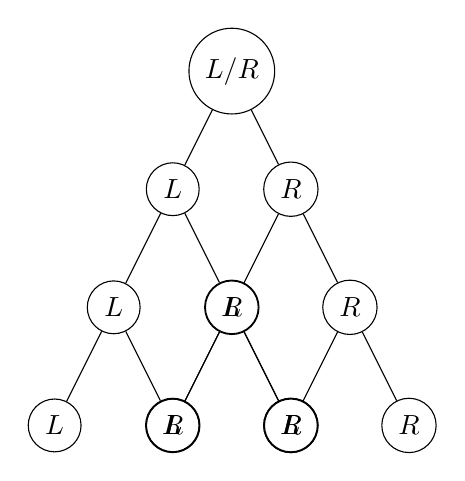
\begin{tikzpicture}
\node[circle,draw](1){$L/R$}
  child {
      node [circle,draw](2){$L$}
         child {
             node [circle,draw](3){$L$}
                   child { node [circle,draw](4){$L$}}
                   child { node [circle,draw](5){$R$}}
         }
         child {
             node [circle,draw](6){$R$}
                   child { node [circle,draw](7){$L$}}
                   child { node [circle,draw](8){$R$}}
         }
   }
   child {
       node [circle,draw](9){$R$}
         child {
             node [circle,draw](10){$L$}
                   child { node [circle,draw](11){$L$}}
                   child { node [circle,draw](12){$R$}}
         }
         child {
             node [circle,draw](13){$R$}
                   child { node [circle,draw](14){$L$}}
                   child { node [circle,draw](15){$R$}}
         }
   };
\end{tikzpicture}
\end{figure}

Suppose we have before us 2 red aces and 2 red kings from the usual deck of 52 cards. How many different pairs consisting of one ace and one king can be put together? Since each ace can be paired with either of 2 kings, there are 2 different pairs for any one ace. Since we have 2 aces, there are $2 \cdot 2$ or 4 different pairs.

\section{Counting selections}
Consider in how many ways can we arrange the set $\{1,2,3\}$:
\[
\{1, 2, 3\}, \{1, 3, 2\}, \{2, 1, 3\}, \{2, 3, 1\}, \{3, 1, 2\}, \{3, 2, 1\}
\]
that is we have $3$ ways of choosing the first element, and $3-1$ options for the second (as we cannot repeat the first choise) and $3-2$ for the last (as non of the former two choices may be used), therefor we can arrange them in $3 \cdot 2 \cdot 1 = 6$ ways. In general we define the number of permutations of a set with $n$ elements as the faculty function $n!$
\[
n! = n \cdot (n-1) \cdot (n-2) \cdots  (n - (n -1)) = 1 \cdot 2 \cdots n = \prod_{k=1}^{n}k,
\]

the last notation simply means that we multiply all the values of $k$ from $1$ to $n$. A recursive version (a self-calling function) can be constructed by noting that $n! = n(n-1)!$. \\

\myindent Now consider a slightly more complex question: in how many ways can we pick two elements from the set $\{1,2,3\}$, the answer turns out to be three ways:
\[
\{1, 2\}, \{1, 3\}, \{2, 3\}
\]
To generalize this we can ask in how many ways can we pick a unordered subset with $k$ elements from a set with $n$ elements ?. To answer this, observe there are $n$ choices for the first element and for each of these there are $n - 1$ choices for the second; and so on until there are $n - k + 1$ for the k'th element. That is we have $n \cdot (n-1) \cdots (n - k + 1)$ ways for picking a $k$-element subset from $n$. As we are picking unordered sets and since each $k$-element subset has exactly $k!$ different orderings, we get our answer by dividing with $k!$:
\begin{equation}\label{binom}
\binom{n}{k} = \frac{n(n-1) \cdots (n - k + 1)}{k!},  \qquad \text{integer } n \geq k \geq 0
\end{equation}
and if we multiply the numerator and denominator of \ref{binom} by $(n - k)!$ we get:
\[
\frac{n(n-1) \cdots (n - k + 1)}{k!} \cdot \frac{(n - k)!}{(n - k)!} =  \frac{n!}{k!(n-k)!}
\]
The symbol $\binom{n}{k}$ is known as a binomial coefficient and we read it "$n$ choose $k$" (the number of ways to select $k$ elements from $n$ element set). Using this result we can directly answer the above question of how many ways to choose two elements from a three element set:
\[
\binom{3}{2}  = \frac{3!}{2! (3-2)!} = \frac{3 \cdot 2 \cdot 1}{2 \cdot 1 \cdot 1} = 3
\]
Interestingly when determining the number of ways to pick $k$ elements we have in effect also specified the $n-k$ unchosen things, therefore
\begin{equation}\label{binom_symmetry}
\binom{n}{k} = \binom{n}{n-k}
\end{equation}
this symmetry can be observed in the above example where we have $3$ ways of picking $2$ elements from a $3$-element set but then also $3$ ways of picking the remaining element. It also follows directly from the definition of the binomial coefficient
\[
\binom{n}{k} =  \frac{n!}{k!(n-k)!} =  \frac{n!}{(n-(n-k))!(n-k)!} = \binom{n}{n-k}
\]

\myindent Another rather remarkable result, known as Pascal's rule, can be derived by marking a particular object $\epsilon$ in an $n$-element set. Now if we pick $k$ objects from $n$, then either $\epsilon$ is picked or it is not. If $\epsilon$ is in the subset then there is $k-1$ objects left to choose among the $n-1$ elements, or more formally $\binom{n-1}{k-1}$. If $\epsilon$ is not in the subset, we need to choose all the $k$ elements in the subset from the $n-1$ objects that are not $\epsilon$; formally that is $\binom{n-1}{k}$. Thus there are
\[
\binom{n-1}{k-1} + \binom{n-1}{k}
\]
ways to choose $k$ elements from $n$ depending on whether $\epsilon$ is included in each selection or not. But this number must be the same as the binomial coefficient and thus we get:
\begin{equation}\label{pascal_rule}
\binom{n}{k}  = \binom{n-1}{k-1} + \binom{n-1}{k}
\end{equation}
this result can also be arrived at by algebraic manipulation
\begin{align*}
 \binom{n-1}{k-1} + \binom{n-1}{k}
& =  \frac{(n-1)!}{(k-1)!((n-1)-(k-1))!} + \frac{(n-1)!}{k!((n - 1) - k)!} \\
& =  \frac{(n-1)!}{(k-1)!(n-k)!} + \frac{(n-1)!}{k!(n - (k + 1))!} \\
& =  \frac{k(n-1)!}{k!(n-k)!} + \frac{(n-1)!(n-k)}{k!(n - k)!} \\
& =  \frac{(n-1)!(k + n - k)}{k!(n-k)!} \\
& =  \frac{n!}{k!(n-k)!}
\end{align*}

%% PASCALs TRIANGLE
\myindent From Pascal's rule we can construct his famous triangle. Observe that according to this rule (see \ref{pascal_rule}) you can calculate $\binom{5}{3}$ as:
\begin{align*}
 \binom{5}{3}
& =  \binom{4}{3} + \binom{4}{2}  \\
& =  \binom{4}{3} + \binom{3}{2} +  \binom{3}{1} \\
& =  \binom{4}{3} + \binom{3}{2} +  \binom{2}{1} + \binom{2}{0} \\
\end{align*}
as $\binom{2}{0} = 1$, we can stop the expansion. In general as $\binom{n}{n}$ and $\binom{n}{0}$ are always $1$ (when $n \geq 0$) we are guarantied that the expansion always terminates. Thus we have found a convenient way of expressing higher binomial coefficients as sums of consecutive smaller ones:
\begin{center}
\begin{tabular}{l|*{5}{c}r}
\toprule
$n$ & $\binom{n}{0}$        & $\binom{n}{1}$ & $\binom{n}{2}$ & $\binom{n}{3}$ & $\binom{n}{4}$  & $\binom{n}{5}$ \\
\hline
0		& 1                     & 0 			       & 0 			        & 0 			       & 0 			         & 0   \\
1   & 1                     & 1 			       & 0 			        & 0 			       & 0  			       & 0   \\
2   & 1                     & 2 			       & 1 			        & 0 			       & 0  			       & 0   \\
3		& 1                     & 3 			       & 3 			        & 1			         & 0  			       & 0   \\
4		& 1                     & 4 			       & 6 			        & 4			         & 1  			       & 0   \\
5		& 1                     & 5 			       & 10 			      & 10			       & 5  			       & 1   \\
\bottomrule
\end{tabular}
\end{center}
discarding the zero's we can arrange these numbers into a triangle:
\[
\begin{array}{c}
1 \\
1\ \myindent 1\\
1\ \myindent 2\ \myindent 1   \\
1\ \myindent 3\ \myindent 3\   \myindent 1   \\
1\ \myindent 4\ \myindent 6\   \myindent 4\   \myindent 1\\
1\ \myindent 5\ \myindent 10\ \myindent 10\ \myindent 5\ \myindent1\\
\ \textnormal{and so on} \ \\
\end{array}
\]
where the next row must contain:
\[
\binom{6}{0} \myindent \binom{6}{1} \myindent \binom{6}{2} \myindent \binom{6}{3} \myindent \binom{6}{4} \myindent \binom{6}{5} \myindent \binom{6}{6}
\]
but we already know that expressions like $\binom{6}{1}$ can be rewritten to
$\binom{5}{1} + \binom{5}{0} = 5 + 1$. So we see that each entry in the new row
is obtained simply by adding the numbers in the row above to the left and right.
\[
1\ \myindent 6\ \myindent 15\ \myindent 20\ \myindent 15\ \myindent 6\ \myindent 1
\]

To generate the triangle, you start with a 1, and then immediately below it, you put two 1’s, one to either side. Then for each successive row, you put a new 1 at either end and complete the row between them by adding together each adjacent pair of entries in the row above and putting their sum halfway between them.

% TODO binomials (a+b)^2 = 1 2 1, (a+b)^3 = 1 3 3 1

\newpage
%%
\section{Newton's Binomial Theorem}
In mathematics a binomial is a polynomial with two terms, i.e such as these
\[\begin{array}{lcl}
(a + b)^0 &=& 1\\
(a + b)^1 &=& a + b \\
(a + b)^2 &=& a^2 + 2ab + b^2 \\
(a + b)^3 &=& a^3 + 3a^2b + 3ab^2 + b^3 \\
(a + b)^4 &=& a^4 + 4a^3b + 6a^2b^2 + 4ab^3 + b^4 \\
:                &   & :
\end{array}\]
or in general
\[
(a+b)^n = \overbrace{(a+b)(a+b)\cdots(a+b)}^{n\textnormal{ factors}}
\]
the relationship between such polynomials and combinatorics stems from the so called binomial theorem.

%\newpage
%\section*{Exercises}
%\addcontentsline{toc}{section}{Exercises}
%\subsection*{Warmups}
% 1
%\begin{exc}\label{ex:analysis:1}
%Show that
%\[
%\binom{n}{0} + \binom{n}{1} + \cdots + \binom{n}{n - 1} + \binom{n}{n} = 2^n
%\]
%\end{exc}
% 2

\section{Exercises}
\begin{ExerciseList}

\Exercise Count the following
\Question A gardening store offers $4 $ different flowers and $4$ different types of pots how many different arrangement of pot and plant can you make
\Question A girl has $3$ hats, $2$ dresses, and $2$ pairs of shoes. How many different costumes does she have?
\Question A deck of $52$ cards contains $4$ different aces and $4$ different kings. How many different pairs of cards, each pair consisting of one ace and one king, can be formed from the aces and kings?
\Question In how many different ways can $7$ people sit in $3$ chairs ?
\Question There are $7$ people in a room. If everyone shakes everyone else's hand exactly once, how many handshakes occur? 
\Answer Using the rules of counting we find
\begin{enumerate}
\item \myindent Each of the four plants can be placed in four different pots yielding $4 \cdot 4 = 16$ possible arrangements
\item \myindent TODO describe why $3 \cdot 2 \cdot 2 = 12$
\item \myindent TODO describe why $4 \cdot 4$
\item \myindent $7$ different ways to pick the first chair, leaving $6$ different people to pick the second chair, leaving $5$ different people to pick the fifth chair i.e. $7*6*5 = 210$
\item \myindent $\frac{7*6}{2}$ handshakes will occur as each of the seven people will shake hands with six other people but since one person shaking with another is counted twice we divide with two.
\end{enumerate}

\end{ExerciseList}


\chapter{Trigonometry}

the  last  great  creation  of  the  Greek  period,  plane  and
 spherical  trigonometry  by  Hipparchus  and  Ptolemy  and  their  application  to
 one  of  the  dreams  of  mankind,  understanding  the  movements  of  the  heavenl bodies.  This  gave  rise  to  modern  astronomy  and  the  physical  sciences.


% TODO missing trig information
% - add figures for and explain why sin, cos and tan exists
% - proove the rrlations between the trig functions

Trigonometric functions are functions of angles. Figure 1.2 shows a right-angled
triangle (ie a triangle with one angle of 90°) with another angle denoted by
the Greek letter theta θ. The sides of the a right-angled triangle are called
the adjacent side (next to θ), the opposite side (opposite to θ) and the
hypotenuse (opposite the right-angle). For any right-angled triangle, the
ratios of the various sides are constant for any particular value of θ. The
basic trigonometric functions are:

\subsection{Trigonometric relations}
\begin{equation}
    tan(\theta) = \frac{sin(\theta)}{cos(\theta)}
\end{equation}

The reciprocals of the $cosine$, $sine$, and $tangent$ are known as
$secant$ ($sec$), $cosecant$ ($csc$), and $cotangent$ ($cot$):
\begin{equation}
    sec(\theta) = \frac{1}{sin(\theta)}
\end{equation}
\begin{equation}
    csc(\theta) = \frac{1}{cos(\theta)}
\end{equation}
\begin{equation}
    cot(\theta) = \frac{1}{tan(\theta)}
\end{equation}

\subsection{Inverse trigonometric functions}

\section{Exercises}
\begin{ExerciseList}
\end{ExerciseList}

\chapter{Analytical geometry}
% TODO missing analytical geometry concepts
% - describe structure of coordinate system
% - describe connections between functions and ordered pair (x, f(x))
% - recreate plane and solids

Analytic geometry, also known as coordinate geometry, or Cartesian geometry, is the study of geometry using a coordinate system.

\section{Coordinate systems}
Coordinate systems are used to uniquely define the position of a point or other geometric or physical object. An everyday use of a coordinate system is the grid reference used to locate places on a map.

% TODO draw picture of map

\subsection{Cartesian coordinate system}
A plane is a flat two-dimensional surface, so Cartesian coordinates in two dimensions are often known as the Cartesian plane.

We define the position of a point, P for example, in terms of its x, y and z coordinates. So if P's position is at x = 2, y = 3, z =4 we say (2,3,4) are the coordinates of P. The coordinates of various points on the Cartesian plane are shown in Figure

% TODO draw two dimensional cartesian coordinate system

The x, y and x, y, z coordinates we've used so far, where the axes (singular - axis, as in ‘the x axis’) intersect at right angles, are known as the Cartesian or rectangular coordinate system, with the point O where the axes intersect called the origin.

% TODO draw tree dimensional cartesian coordinate system

\subsection{Polar coordinate system}
Although Cartesian coordinates are a nice, simple coordinate system, they aren't so suitable when circular, cylindrical, or spherical symmetry is present. In those circumstances, in two dimensions, plane polar coordinates are a better choice, where the position of a point on the plane is given in terms of the distance r from a fixed point and an angle θ from a fixed direction (see Figure 1.10). So, if point P was a distance r = 6 from the origin, and the angle θ = 120°, the coordinates of P would be (6, 120°).

% TODO draw example and show how to convert between coordinate systems

\subsection{Spherical coordinate system}
In three dimensions, the position of a point P in space can be defined using spherical coordinates (r, θ, ϕ) as shown in Figure 1.12. To go from spherical coordinates to Cartesian coordinates we see that

% TODO draw example and show how to convert between coordinate systems

% EXCERCISES
% - Graph the circle (x+3)^2+(y+2)^2=9.

\section{Exercises}
\begin{ExerciseList}
\end{ExerciseList}

\chapter{Calculus}
% TODO missing calculus concepts
% http://www.science4all.org/le-nguyen-hoang/infinite-series/
% - Area under curve
% - Fundamental theorem of calculus
% - Proof and explain taylor series
% - Proof Finite geometric series https://www.khanacademy.org/math/precalculus/seq_induction/geometric-sequence-series/v/geometric-series-introduction
% - Numerical integration http://rosettacode.org/wiki/Numerical_integration#ActionScript
% - LaplaceTransform http://reference.wolfram.com/language/ref/LaplaceTransform.html
% - story of e (proof the limit of the series)
% - relationship between pi, e and i
% - include info on e from "the story of e"
% - include info on i from  "the story of i"
% Gamma function and Stirling's approximation
% TODO eulers identity
% general binomial theorem (the binomial theorem for fractional and negative powers).
% https://medium.com/fintechexplained/calculus-2-a-must-know-concept-for-every-professional-a86599caa2a5

% TODO rewrite
Differentiation: Helps us understand how an output of a function changes when its inputs change. This article will concentrate on the concept of differentiation.
Integration: Helps us calculate the total impact of the change over time and helps us compute a function from its derivative. The next article will outline the concept of integration.
Rate of change is a measure of how much a quantity changes (increases or decreases) in relation to the change in another quantity.
Derivative of a function measures how sensitive an output of a function is to the input of the function. Differentiation is the name of the process in which a set of steps are performed to find the derivative of a function.

Example
Let’s consider that a variable y depends on a variable x. For instance, y could be the speed of a football player kicking a ball and x could be the number of hours the player spent in the training camp.
Let’s now start recording the ball speed and the number of hours the players spent in the training camp. Let’s also record whether they are left footed or right footed by the sign of x: negative sign implies that the player is left footed and position sign means that the player is right footed:
When x=-4, y =16.
When x =-3, y =9
When x=0, y =0.
When x =1, y =1.
When x =2, y = 4.
When x =3,
When x= 10, y = 100
When x = -11, y = 121
If we plot the chart where y points are plotted on the y axis and x points are plotted on the x-axis then we’ll see a y = x² chart:

We could pick a point on the chart (x,y), draw a line tangent to the chart and take our rate of change as change in y over change in x. We would then repeat this exercise for all points on the chart and calculate the average of the gradient.
Tangent is a strange line that aims to have the same gradient as the curve.

Rate of change (or gradient) = difference in y / difference in x = dy/dx

Slope is also known as the gradient of a chart

The gradient at point (x1,y1) and (x2,y2) will be completely different from the gradient at point (y4,x3) and (x2, y2).
We could instead use the techniques of calculus and utilise differentiation to find the instantaneous rate of change. Differentiation will enable us to find the rate of change of value of y when the value of x changes by a very small unit. Derivative is essentially finding the rate of change in the function when we change the value of x.

We understood that derivative is all about finding how fast/slow the output of a function changes when we change the input of the function. Therefore, we can start changing the value of x by 1 unit and start seeing how the value of y changes. Or, we could plot the chart and pick any of the two points on x axis, then find the value of y and then calculate the slope.
Let’s refer to the small increment to the input in x as Z.
Therefore, the function f(x) becomes: f(x + Z) implying that we are adding Z to the value of x.

rate of change (or gradient) = (f(x + Z) - f(x))/(x+Z-x)

This is known as Newton’s difference quotient.

the power rule.
d/dx x^a = a * x^(a-1)
Therefore: If f(x) = x² Then its derivative is 2x

Second Order Differentiation:
It merely means repeating the differentiation twice. Differentiating a function returns a new function. Second order differentiation is about calculating the derivative of the derivative:

% Excercises
% - derivatie of x^3 = 3x^2
% - derivatie of 3x^2 = 6x

\section{Logarithms}
If I'm driving at a constant velocity, say 60 km per hour, the distance I travel is changing in a constant manner, ie every hour I cover 60 km. We can say the rate of change of the distance I travel with respect to time is constant. However, if my car is moving with constant acceleration, its velocity is changing in a constant manner, but the distance I travel is not changing constantly - because I'm accelerating. We can say the rate of change of the distance I travel, with respect to time, is not constant.

\section{Differential calculus}
Differential calculus allows us to find the exact slope of a curve, in other words a function's rate of change, at any particular point. We are assuming that the function is differentiable in the first place and that the gradient doesn't go shooting off to infinity.
\[
\frac{f(x + \Delta x) - f(x)}{\Delta x}
\]
is known as the difference quotient, or the Newton quotient, and its limit defines the derivative of a function.


\subsection{The derivative}
This limit is known as the derivative and is the heart of differential calculus. In this example, where $y = x^2$ the derivative could be denoted by
\[
\frac{dy}{dx}
\]

\[
f(x) = x^k 
f'(x) = kx^{k-1}
\]

\subsubsection{the product rule}
We use this rule when differentiating a product of two or more functions.

\subsubsection{the chain rule}
The chain rule This rule is used if a function is a function of another function. So, if y is a function of u and u is a function of x, then the derivative of y with respect to x is equal to the derivative of y with respect to u multiplied by the derivative of u with respect to x,

\section{Integral calculus}
For example, say we have a function that tells us the acceleration of an object after a certain time. If we can integrate that function we obtain a new function that tells us the velocity of the object after a certain time. If we integrated the second function, we'd get a third function that tells us the distance covered after a certain time. But we can also do that sequence of calculations in reverse, by starting with the function that tells us distance covered after a certain time. We can differentiate that function to find the object's velocity and differentiate again to find its acceleration.

% TODO explain why distance, velocity and accelaration is so inter linked (explain physical formulas)
% Hermite’s method
\subsection{Laplace Transform}


\section{Sequences}
A \index{Sequences}{sequence} is a ordered list of things (usually numbers) for example $\left\{1, 3, 5, 7\right\}$ is the finite sequence of the first $4$ odd numbers. and $\left\{1, 2, 4, 8, 16, 32, ...\right\}$ is an infinite sequence where every term doubles. When the sequence goes on forever it is called an infinite sequence, otherwise it is a finite sequence. Sequence is like a \index{Set}{set} except the terms are in order (with sets the order does not matter) and the same value can appear many times (only once in Sets). For example $\left\{0, 1, 0, 1, 0, 1, ...\right\}$ is the sequence of alternating $0$s and $1$s, the set is just $\left\{0,1\right\}$.

To make it easier to use rules, we often use this special style:

\section{Series}
A \index{Series}{series} is, informally speaking, the sum of the terms of a sequence.

\subsection{Taylor series}
\begin{equation}
cos(\theta) = \sum_{n=0}^{\infty} \frac{(-1)^n \cdot \theta^{2n}}{2n!}
\end{equation}

\subsection{Geometric Series}
\begin{equation}
a + ar + ar^2 + ar^3 + \cdots + ar^{n-1} = \sum_{k=0}^{n-1}ar^k = a \frac{1-r^n}{1-r}
\end{equation}

% artimetic series http://www.mathsisfun.com/algebra/sequences-sums-arithmetic.html


\section{Special functions}
\subsection{Logarithm}
A logarithm (log or logs for short) goes in the opposite direction to a power by asking the question: what power produced this number? So, if 2x = 32, we are asking, ‘what is the logarithm of 32 to base 2?’ We know the answer: it's 5, because 25 = 32, so we say the logarithm of 32 to base 2 is 5. In general terms, if , then we say the logarithm of a to base x equals p, or For example, 104 = 10,000, so we say the logarithm of 10,000 to base 10 equals 4, or We can take logarithms of any positive number, not just whole ones. So, as 103.4321 = 2704.581 we say the logarithm of 2704.581 to base 10 equals 3.4321, or Logarithms to base 10 are called common logarithms. Older readers may remember, many years ago - after the dinosaurs, but before calculators and computers were widely available - doing numerical calculations laboriously by hand using tables of common logarithms and anti-logarithms. The properties of logarithms are based on the aforementioned rules for working with powers. Assuming that a > 0 and b > 0 we can say: logx(ab) = logxa + logxb, eg log10(1000 × 100) = log10(100,000) = 5 = log10(1000) + log10(100) = 3 + 2. logx(1/a) = -logxa, eg log3(1/27) = -log327 = -3. logx(a/b) = logxa - logxb, eg log2(128/8) = log2(16) = 4 = log2(128) - log2(8) = 7 - 3. logx(ay) = ylogxa, eg log5(253) = log515,625 = 6 = 3 × log525 = 3 × 2. 1.8.3

% TODO algorithms for calculating logarithms (Taylor series) http://en.wikipedia.org/wiki/Logarithm#Power_series

\subsection{Natural logarithm}
% TODO plot y = ln{x} and add as compound ingerest in index (use correct symbols as used in compound intersts)
% the area under the hyperbola y = 1/x —led independently to the same number, leaving the exact origin of e shrouded in mystery.
Say we invest 1 in a bank that pays 100\% interest per year. If the bank calculated and credited the interest at the end of one year, our investment would then be worth $1 + 1 = 2$. But if the bank credits the interest more frequently than once a year say every six months, at the end of that period the balance would equal $(1 + 1/2)$ since we would get half of the yearly interest payed each six months. At the end of one year the total amount would be $(1 + 1/2)(1 + 1/2) = (1 + 1/2)^2$ as the interest (compund or basic). Calculated three times a year after four moths we would have $(1 + 1/3)$ after eight $(1 + 1/3)^2$ and the final balance would be $(1 + 1/3)^3$. In general, if interest is calculated n times a year, the balance after one year is
\[
f(k) = \left(1 + \frac{1}{k}\right)^k
\]
if we plug in some values we observe
\[
\begin{align*}
  f(2)  =& \left(1 + \frac{1}{2}\right)^2 = 2.25 \\
  f(5)  =& \left(1 + \frac{1}{5}\right)^5 = 2.248832 \\
  f(10) =& \left(1 + \frac{1}{10}\right)^{10} = 2.59374...
\end{align*}
\]

n 
1 2 
2 2.25 
3 2.37037 
4 2.44141 
5 2.48832 
10 2.59374 
100 2.70481 
1000 2.71692 
100,000 2.71827 
1,000,000 2.71828 
10,000,000 2.71828

We can see that as n increases, the value of the function appears to settle down to a number approximately equal to 2.71828. It can be shown that as n becomes infinitely large, it does indeed equal the constant e. The mathematically succinct way of saying this introduces the important idea of a limit and we say where means the limit of what follows (ie ) as n approaches infinity (symbol ). In other words, e approaches the value of as n approaches infinity.

\begin{equation}
e = \lim_{k\to\infty}\left(1 + \frac{1}{k}\right)^k
\end{equation}

\subsection{The exponential function}
% TODO plot y=e^x
The exponential function f(x) = ex, often written as exp x (see Figure 1.7) arises whenever a quantity grows or decays at a rate proportional to its size: radioactive decay, population growth and continuous interest, for example. The exponential function is defined, using the concept of a limit, as

\section{Exercises}
\begin{ExerciseList}
\end{ExerciseList}

\chapter{Modern Algebra}

\section{Complex numbers}

\chapter{Numerical analysis}
% TODO missing numerical concepts
% - Compare with Archimedes calculations of PI
% - Babylonian method http://en.wikipedia.org/wiki/Methods_of_computing_square_roots#Babylonian_method
% - Runge–Kutta for ordinary differential eqautions http://en.wikipedia.org/wiki/Runge–Kutta_methods
% - Newton rapson method for square roots http://www.sosmath.com/calculus/diff/der07/der07.html
% - Finite difference methods (check "Finite difference methods in Finance" book on OneFrive)
% - Trapez integration
Already the Babylonians knew how to approximate square roots, their method was based on simple process of continuously improving guesses. For example to find $\sqrt{10}$ we may guess $3$ then square it to get $9$, as this is less than 10 we know $3 < \sqrt{10}$ next we may guess $4$ which squares $16$ as this is above $10$ we know now $3 < \sqrt{10} < 4$. For our next guess we may take the mean of the boundaries $3$ and $4$ resulting in $(1/2 \times (3+4))^2 = (7/2)^2 = 49/4$ as $49/4 > 10$ we now know that $3 < \sqrt{10} 7/2$. Applying the last step again we find $(1/2 \times (3 + 7/2))^2 = (13/4)^2 = 169/16$ which again is above $10$ so now we know $3 < \sqrt{10} 13/4$ and so on.

However this method seam crude and tedious to carry out by hand, to improve it we need to get better at guessing which numbers are good candidates for approximations of the square root of a number $n$. To do this lets examine the nature of $\sqrt{n}$. Informally if we assume $(n/2)^2 < n$ for $n>0$ then
\[
(n/2)^2 < n \rightarrow n^2/4 < n \rightarrow n < 4
\]
so for positive numbers less than $4$ our initial guess has to be above half $n$ (the approximations lower bound is $n/2$). Conversely if we assume $(n/2)^2 > n$ for $n>0$ then
\[
(n/2)^2 > n \rightarrow n^2/4 > n \rightarrow n > 4
\]
S
That is for numbers above $4$ our initial guess has to be below half $n$ (the approximations upper bound is $n/2$).

\section{The Newton-Raphson Method}
The Newton-Raphson Method

\subsection{Roots}

\section{Approximating differential equations}
\subsection{Finite-difference methods}

\section{Numerical integration}

\section{Exercises}
\begin{ExerciseList}
\end{ExerciseList}

\chapter{Linear algebra}
% TODO missing linear algebra concepts
% - http://resources.codingthematrix.com
% - http://en.m.wikipedia.org/wiki/Perron–Frobenius_theorem
% - spectral theorem https://inst.eecs.berkeley.edu/~ee127a/book/login/l_sym_sed.html
% - discrete fourier transform http://jeremykun.com/2012/06/23/the-discrete-fourier-transform/
% - fast fourier transform http://jeremykun.com/2012/07/18/the-fast-fourier-transform/
% - http://www.physicsclassroom.com/class/vectors/Lesson-1/Vector-Addition

% field
Real numbers \\
Complex numbers\\
Finie field GF2

% vectors
Vectors \\
Vector addition
Vector scalar multiplication
Convex combinations
Affine combinations
Dot product 
Solving triangular systems

% vector space
Linear combination
Span
Vector spaces
Afine spaces
Linear systems, homogenous and otherwise

% Matrix
Rows, columns and entries
identity matrix
Column space and row space
Matrix vector and vector matrix multiplication
 - dot products
 - linear combinations
Null space
Sparse matrix
Linear functions
Matrix matrix multiplication
Column vector 
Row vector
inner product 
outer product
Matrix inverse

% The basis
Minimum spanning forest

% Dimension
Dimension and rank

% Gausian eleminiation
Echelon form
Solving vector matrix equations
Factoring integers

% The inner product
Distance, length, norm and inner product
Orthogonality

% Orthogonalization
QR factorisation
Least squares
Line fitting

% Special bases
Wavelets
Fourier transform
Discrete foruer transform

% Singular value decomposition
Low rank matrixes

% The eigenvector
Discrete dynamic processes
Diagonalisation and the Fibonacci matrix
Eigen values and eighen vectors
Markov chains

% Linear programming
Geometry of linear programming
The simplex algorithm
Game theory


\[ 
\norm{a \vec{u}} = \abs{a} \, \norm{\vec{v}} 
\]

\section{Vectors}
numbers. Another example: when representing, say, a  1024×768 black-and-white image as a vector, we define the vector as a function from the domain $D = {1,..., 1024} × {1, .., 768}$ to the real numbers. The function specifies, for each pixel $(i, j)$, the image intensity of that pixel. 

% vector dot product
\begin{description}
    \item[Addition]
    \item[Inner product (dot product)]
    \item[Pointwise vector division]
    \item[Pointwise vector multiplication]
    \item[Saxpy]
    \item[Scalar vector multiplication]
\end{description}

\section{Matrices}
% http://www.eng.buffalo.edu/Research/BEST/Research/Lecture%20Series%202013/Matrix%20Multiplication.pdf
% transpose http://www.mathwords.com/t/transpose_of_a_matrix.htm
% inverse http://www.mathwords.com/i/inverse_of_a_matrix.htm
\begin{description}
    \item[Addition]
    \item[Pointwise matrix division] (denominator matrix must have non-zero entries)
    \item[Pointwise matrix multiplication]
    \item[Rank] The rank of a matrix is the number of linearly independent columns (which is equal to the number of linear independent rows)
    \item[Scalar matrix multiplication]
\end{description}

\section{Exercises}
\begin{ExerciseList}
\end{ExerciseList}

\chapter{Sets and functions}
% TODO Sets missing concepts
% - union, complement and intersection of sets
% - filtered set, unordered sets, ordered set
%\section{Naive set theory}
%\section{Counting the Infinite}
%\subsection{Problems with naive set theory}
%\section{Axiomatic set theory}
%\section{Cantor and the Transfinite Realm}
% Morphism In many fields of mathematics, morphism refers to a structure-preserving mapping[disambiguation needed] from one mathematical structure to another.
% Set builder notation
% Power set
%
%- Operations
%    - Equivalence
%    - Converse
%    - Implication
%- Functions
%    - Map
%    - Injective
%    - Bijective
%    - Surjective
%    - Inverse

\section{Sets}
%. TODO rewrite
A set is a collection of objects, and a function is an association of members of one set to members of another. Most high-level mathematics is about sets and functions between them. For example, calculus is the study of functions from the set of real numbers to the set of real numbers that have the property that we can differentiate them. In effect, we can view sets and functions as the mathematician’s building blocks.

(We don’t care about the ordering of the list. nor about duplicates so {1,2} is the same set as {2,1} which is the same as {2,1, 2}) If x is a member of the set X, then we write x ∈ X. We read this as ‘x is an element (or member) of X’ or ‘x is in X’.3 If x is not a member, then we write x ∉ X .

The set containing the numbers 1, 2, 3, 4 and 5 is written {1, 2, 3, 4, 5}. The number 3 is an element of the set, i.e. 3 ∈ {1, 2, 3, 4, 5}, but 6 ∉ {1, 2, 3, 4, 5}. Note that we could have written the set as {3, 2, 5, 4, 1} as the order of the elements is unimportant.

The set {1, 5, 12, {dog, cat}, {5, 72}} is the set containing the numbers 1, 5, 12 and the sets {dog, cat} and {5, 72}. Note that sets can contain sets as members.

It is vitally important to note that {5} and 5 are not the same. That is, we must distinguish between being a set and being an element of a set. Confusion is possible since in the last example we have {5, 72}, which is a set in its own right but can also be thought of as an element of a set, i.e. {5, 72} ∈ {1, 5, 12, {dog, cat}, {5, 72}}.

% TODO write this out as a defenition with a number
% A set is a well-defined collection of objects.2 The objects in the set are called the elements or members of the set.

Loosely speaking a set is a collection of well defined objects. 

    - Cardinality - number of elements in the set
    - X in y
    - X !in y
    - Sets can contain other sets
    - Two sets are equal if they contain the same elements {1,2} = {2,1,2} (order and repetitions are not important)
    - x subset y - every element of x is in y
    - x proper-subset y - every element of x is in y and x is not equal to y
    - x union y = x in X or x in Y (or x in both)
    - x intersect y = x in X and x in Y
    - x \ y = x in X and x !in y (if y subset x then x\y is complement of y in x)
    - (a,b) - interval greater than a and less than b
    - [a,b] - interval from a to b (both included)
    - X x Y - set product is all pairs (x,y) where x in X and y in Y

Some common operations on sets
\begin{description}
\item[Empty set] $\varnothing = \{\}$.
\item[Set intersection] $S \cap T$ is the set containing all the elements that are in both $S$ and $T$:
\begin{equation}
S \cap T := \left\{{x: x \in S \land x \in T}\right\}
\end{equation}
\item[Set union] $S \cup T$ is the set containing all the elements that are in either or both of the sets $S$ and $T$:
\begin{equation}
S \cup T := \left\{{x: x \in S \lor x \in T}\right\}
\end{equation}
\item[Cardinality] For finite sets A and B, |A × B| = |A|·|B|. 
% TODO include algorithm
\end{description}

A indexed set is a collection of values associated with indices. For example
\begin{itemize}
\item An ordered pair is a family indexed by the two element set $2 = \{1, 2\}$.
\item An n-tuple is a family indexed by $n$.
\end{itemize}
the set that whose members label (or index) members of a family is called an index set. 

\section{Functions}
% TODO consider merging with input from "thinking like a mathematician"
Loosely speaking, a function is a rule that, for each element in some set D of possible inputs,  assigns a possible output. The output is said to be the image of the input under the function 

For a function named f, the image of q under f is denoted by f(q). If r = f(q), we say that  q maps to r under f. The notation for “q maps to r” is q )→ r. (This notation omits specifying  the function; it is useful when there is no ambiguity about which function is intended.)  It is convenient when specifying a function to specify a co-domain for the function. The  co-domain is a set from which the function’s output values are chosen. Note that one has some  leeway in choosing the co-domain since not all of its members need be outputs.  The notation  f : D −→ F  means that f is a function whose domain is the set D and whose co-domain (the set of possible  outputs) is the set F. (More briefly: “a function from D to F”, or “a function that maps D to F.”) 

Consider the function prod that takes as input a pair of integers greater than  1 and outputs their product. The domain (set of inputs) is the set of pairs of integers greater  than 1. We choose to define the co-domain to be the set of all integers greater than 1. The  image of the function, however, is the set of composite integers since no domain element maps  to a prime number. 

\subsection{Identity function} 
For any domain D, there is a function idD : D −→ D called the identity function for D, defined  by  idD(d) = d  for every d ∈ D. 

\subsection{Composition of functions}  
The operation functional composition combines two functions to get a new function. We will later  define matrix multiplication in terms of functional composition. Given two functions f : A −→ B  and g : B −→ C, the function g ◦f, called the composition of g and f, is a function whose domain  is A and its co-domain is C. It is defined by the rule  (g ◦ f)(x) = g(f(x))  for every x ∈ A.  If the image of f is not contained in the domain of g then g ◦ f is not a legal expression.  Example 0.3.10: Say the domain and co-domains of f and g are R, and f(x) = x + 1 and  g(y) = y2. Then g ◦ f(x)=(x + 1)2. 

show that composition of functions is associative:  

Proposition 0.3.12 (Associativity of composition): For functions f, g, h,  h ◦ (g ◦ f)=(h ◦ g) ◦ f 
% TODO proof
Let x be any member of the domain of f.  
(h ◦ (g ◦ f))(x) = h((g ◦ f)(x)) by definition of h ◦ (g ◦ f))  
                 = h(g(f(x)) by definition of g ◦ f  
                 = (h ◦ g)(f(x)) by definition of h ◦ g  
                 = ((h ◦ g) ◦ f)(x) by definition of (h ◦ g) ◦ f 
                 
functional inverse of h as well.  In general,  Definition 0.3.13: We say that functions f and g are functional inverses of each other if  • f ◦ g is defined and is the identity function on the domain of g, and  • g ◦ f is defined and is the identity function on the domain of f.  Not every function has an inverse. A function that has an inverse is said to be invertible.  Examples of noninvertible functions are shown in Figures 2 and 3  Definition 0.3.14: Consider a function f : D −→ F. We say that f is one-to-one if for every  x, y ∈ D, f(x) = f(y) implies x = y. We say that f is onto if, for every z ∈ F, there exists  x ∈ D such that f(x) = z. 

\section{Exercises}
\begin{ExerciseList}
% TODO rewrite sample
%\Exercise What is the cardinality of {1, 2, 3,..., 10, J, Q, K} × {♥, ♠, ♣, ♦}? 
%\Answer The cardinality of the first set is 13, and the cardinality of the  second set is 4, so the cardinality of the Cartesian product is 13 · 4, which is 52. 
\end{ExerciseList}

\chapter{Basic probability}
% TODO missing probability concepts
% http://sahilmohnani.wordpress.com/2013/06/03/the-multinomial-and-poisson-distributions/
% - http://sahilmohnani.wordpress.com/2013/06/03/the-chi-square-distribution/
% - Stem-and-leaf plot example http://www.purplemath.com/modules/stemleaf.htm
% - Statistical vs non statistical questions (average vs deterministic)
% - probability models (should probabilities sum to 1)
% Normal distribution https://www.mathsisfun.com/data/standard-normal-distribution.html and https://statistics.laerd.com/statistical-guides/normal-distribution-calculations.php
% - area under the curve
% - http://www.countbayesie.com/blog/2015/3/17/interrogating-probability-distributions
% PDF http://en.wikipedia.org/wiki/Probability_density_function

% - http://jeremykun.com/2013/01/04/probability-theory-a-primer/
% - http://jeremykun.com/2013/03/28/conditional-partitioned-probability-a-primer/
% - http://jeremykun.com/2014/03/03/martingales-and-the-optional-stopping-theorem/
% “law of large numbers,” a major result in the theory of probability. The law of large numbers gives the precise mathematical result that corresponds to the well-known fact that the relative frequency of an event will more accurately predict the likelihood of its occurrence the more trials you observe.

# TODO missing problems to introduce
# - Birthday paradox The question is, How many randomly selected people do you need to assemble in a room for there to be a better-than-even chance that two of them will have the same birthday? The most common answer is 183, just over one-half the number of days in a year. The correct answer is 23. The exact calculation is a bit intricate, but you get a sense of why the answer is so low when you realize that with 23 people, there are 23 × 22 = 506 possible pairs, each of which might share a birthday, and this turns out to be just enough pairs to tilt the odds to 0.508 in favor of there being a match.
# - formal math for montey hall.

% Odds and expectation
% The law of large numbers
% counting rules
% binominal distribution
% normal disttibution
% monte carlo
% game theory

Odds are used by casinos, racetracks, and other gambling establishments to determine payoffs when bets are made. For example, at a race, the odds that a horse wins the race may be 4 to 1. In this case, if you bet $1$ and the horse wins, you get $4$. If you bet $2$ and the horse wins, you get $8$ and so on. suppose you roll a die and if you roll a 3, you win. what amount should you win if you bet 1 on average you win once in every six rolls. So if you lose on the first five rolls and win on the sixth, you have lost $5$; therefore, you should get $5$ if you win on the sixth roll, thus the odds 1 go 5 In gambling games, the odds are expressed in reverse order. For example, if there is one chance in six that you will win, the odds are 1 to 5, but in general, the odds would be given as 5 to 1. In gambling, the house (the people running the game) will offer lower odds, say 4 to 1, in order to make a profit. In this case, then, the player wins on average one time in every six rolls and spends on average $5$, but when the player wins, he gets only $4$. So the house wins on average $1$ for every six rolls of the player. If the odds of winning the game are 1:5, then the odds of losing are 5:1.

One die is rolled; what are the odds in favor of getting a 5 or 6? (1:2)

\begin{equation}\label{prob:odds}
P(event) = \frac{\text{Number of outcomes in favor event}}{\text{Number of outcomes not in favor of event}}
\end{equation}

% reducing sample space
Find the probability of getting a sum of 5 if it is known that the sum of the spots on the dice was odd. There are four ways to get a sum of 5. They are (1, 4), (2, 3), (3, 2), (4, 1), and there are 18 ways to get a sum that is odd; hence, P(sum of 5|sum is odd)= 4/18 alternativly we can use the formula P(sum of 5 and sum is odd) = P(sum of 5) * P(sum is ods|sum of 5) = 4/36 * 1 (as its certain the sun is odd if it was five) 4/36/(1/2) = 4/18

$4/36 * 18/36$

the addition rules. Here one is interested in finding the probability of one event or another event occurring. In these situations, you must consider whether or not both events have common outcomes.
% TODO use black or a 7 card example to show outcomes counted twice
what is the probability that the card is a king or a queen? = mutual exclusive as card cannot be both king and queem thus prob is 4/52 + 4/52 however what is the probability that the card is a king or a diamond = not mutual exclusive as card could be king of diamons = 13 + 4 - 1/52

If A and B are two events that are not mutually exclusive, then P(A or B) = P(A) + P(B) − P(A and B), where A and B means the number of outcomes event A and event B have in common. Adie is rolled. Find the probability of getting an odd number or a number less than 5. $3/6 + 4/6 - 2/6 = 5/6$
For the mathematical purist, only one addition rule is necessary, and that is   P(A or B) = P(A) + P(B) − P(A and B)   The reason is that when the events are mutually exclusive, P(A and B) is equal to zero because mutually exclusive events have no outcomes in common.

% TODO add to index: dependent, independent, mutually excluaive, classical and emperical probabikity, odds, expecgation
Two events, A and B, are said to be independent if the fact that event A occurred does not affect the probability that event B occurs. For example, if a coin is tossed and then a die is rolled, the outcome of the coin in no way affects the outcome, or changes the probability of the outcome, of the die. the first event in some way changes the probability of the occurrence of the second event, the two events are said to be dependent. For example, suppose a card is selected from a deck and not replaced, and a second card is selected. In this case, the probability of selecting any specific card on the first draw is , but since this card is not replaced, the probability of selecting any other specific card is since there are only 51 cards left.

only one multiplication rule is necessary for two events, and that is   P(A and B) = P(A) · P(B|A).   The reason is that when the events are independent, P(B|A) = P(B),

when two independent events occur in sequence, the probability that both events will occur can be found by multiplying the probabilities of each individual event.

% TODO solve using both sample space ans multiplicatiin rule (getting two heads and head on coind + 4 on die)

Probabilities can be computed for situations that do not use sample spaces. In these cases, frequency distributions are used and the probability is called empirical probability.
\begin{equation}\label{prob:frequency-event}
P(event) = \frac{\text{Frequency of event}}{\text{Sum of all frequencies}}
\end{equation}

Another aspect of empirical probability is that if a large number of subjects (called a sample) is selected from a particular group (called a population). we can never know the exact probability for the population onlyy for the sample, however if the sample is representative of the population, the estimate will usually be fairly close to the exact probability. Statisticians have a way of computing the accuracy (called the margin of error) for these situations.
% TODO aplit sectiins between classical and emperical probability
% - create example from mortality table
% - probability to live
% 50 or older
% Under 30 years old
% Between 40 and 59 years old
% Under 60 but over 29 years old




Probability theory is the basis on which statistics and with it a many of mathematics most useful applied subjects rest upon. The ability to calculate probabilities transformed statistics from mere data collection to using data to make informed decisions. Today politicians try to predict voter behavior through opionen polling. Marketing departments study customers to figure out how best to launch new products and in medicine statistics is used to compare the benefits drugs with their risks.

\myindent In spite of their obvious usefulness, probability and statistics are rather new branches of mathematics. Some of the earliest studies of probability comes from gambling. In the sixteenth century Gerolamo Cardano\index{Gerolamo Cardano} demonstrated the efficacy of defining odds as the ratio of favorable to unfavorable outcomes. Later these ideas was picked up and expanded upon by Pierre de Fermat\index{Pierre de Fermat} and Blaise Pascal\index{Blaise Pascal}. In recent years the study of probability and statistics has gained pace as computers allows us to perform studies on ever larger samples.

\myindent In 1494 Luca Pacioli\index{Luca Pacioli} first published the challenge that let Pascal and Fermat to undertake the formal study of probability. The challenge is known as the problem of the unfinished game. Suppose two players $\{A, B\}$ bets on who will win the best of five coin tosses, but then have to stop before either player has won. How do they divide the pot?. If each has won the same number of throws then the pot is split evenly. But what if they stop after three throws, with player $A$ ahead $2\text{-to-}1$?. Pacioli, suggested that the solution is to divide the pot according to the current state of play, namely $2\text{-to-}1$. But in $1539$ Cardano demonstrated that this is incorrect as splitting the pot depended not on how many rounds each player had already won but on how many each player must still win in order to win the contest. To see this consider that as $A$ is ahead $2\text{-to-}1$, the first three rounds must have yielded two heads and one tail. The remaining two throws can yield $\{H,H\}$, $\{H,T\}$, $\{T,H\}$, $\{T,T\}$. In the first scenario $\{H,H\}$, the final score is four heads and one tail, so player $A$ wins; in the second and the third ($\{H,T\}$ and $\{T,H\}$), the final outcome is three heads and two tails, so again player $A$ wins. Only in the fourth scenario with $\{T,T\}$ is the final outcome two heads and three tails, so player $B$ wins. This means that player $A$ wins in three of the four possible ways the game could have ended and thus the pot should be divided $3/4$ for $A$ and $1/4$ for for $B$.

\section{Classical probability}
\epigraph{"I can as easily throw one, three or five as two, four or six. The wagers there are laid in accordance with this equality if the die is honest."}{\textup{Gerolamo Cardano}, Liber de ludo aleae (Book of Games of Chance)}

In the quote above Cardano states that with a fair die the probability of getting $\{1,3,5\}$ is the same as getting $\{2,4,6\}$. He thus formulated one of the earliest known examples of the probability of an event as a fraction: the number of events that meets a constraint (such as a die being even or odd) divided by the total number of possible outcomes (such as the six different faces of a die).
\begin{equation}\label{prob:formula}
P(event) = \frac{\text{Number of events that meet constraint}}{\text{Number of equally likely events}}
\end{equation}
For example a toss of a fair coin has a set of two possible outcomes $\{H,T\}$ known as its \index{sample space}sample space with each possible outcome of the sample space having likelihood $1/2$ of occurring ($50$ percent chance of head or tails). So the probability of the event heads occurring is $P(H) = 1/2$. Similarly a toss of a die has a sample space consisting of $6$ equally likely possible outcomes $\{1, 2, 3, 4, 5, 6\}$ so the probability of the die showing six is $P(6) = 1/6$.

When constructing a sample space for a probability experiment such as drawing cards, throwing dice or flipping coins its important to assign probabilities to all possible outcomes and the sum of these should be exactly $1$. Further the probability of a event will always be a number from $0$ to $1$, where $0$ means that a event cannot occur (such as throwing $7$ with a die) and $1$ means that a event is certain to occur (such as getting a number less than $7$ with a die). The events described above are called simple events\index{Simple event} as they consists of one outcome. When an event consists of more than one outcome it's called a compound event. The probability of getting an odd number when a die is rolled is a compound event as there are three outcomes $1, 3$ and $5$ from the sample space that matches the event. On the other hand if two coins are tossed, the event of getting two heads is a simple event as there is only one way to get two heads with two coins.

\subsection{Product rule}

Cardano next observed that the probability of getting a certain outcome on two successive throws is the square of the probability of getting it on a single throw. For example, the probability of getting double $6$ is $1/6 \times 1/6 = 1/36$, this can be readily seen as the sample space consist of all the 36 enumerations of the possible ways two dice can be rolled and only one of these outcomes is double $6$ (see chapter \ref{combi} for a intro to combinatorics)

Similarly, the probability of getting three even numbers is $1/2 \times 1/2 \times 1/2 = 1/8$ (this assumes that is the events are \index{Independent event}independent events, i.e. that the first throw does not influence the second). That is the probability of two independent events $A$ and $B$ both occurring is
\begin{equation}\label{prob:compound-event}
P(A \text{ and } B) = P(A) \times P(B)
\end{equation}
With multiple independent events occurring the probability off all of them occuring is the product of the likelihood of each individual event. So, if the probability of you finishing this chapter is $9/10$, and the probability of you finishing the next one is also $9/10$, then the total probability of you finishing both chapters isn't $9/10$ but instead $9/10 \times 9/10 = 81/100$. Note if you remove the restriction on the order in which the events occurs then there are more possibilities. For example, the probability of rolling a $6$ followed by an even number is $1/6 \times 1/2 = 1/12$ but without the restriction of order it becomes $5/36$. The easiest way to see this is to count all the possible outcomes of throwing two dies $6 \times 6 = 36$ and then count the number of favorable outcomes (the die is even or six) $\{2,6\}$, $\{6,2\}$, $\{4,6\}$, $\{6,4\}$, and $\{6,6\}$. As there are five such outcomes we arrive at $5/36$.

\myindent Cardano next considered examples where we are interested in any of two \index{Mutually exclusive event} mutually exclusive events. That is two events that cannot occur at the same time, such as getting heads and tails on the same coin flip i.e $P(H \text{ and } T) = 0$. He observed that given
\begin{equation}\label{prob:exclusive-event}
P(A \text{ or } B) = P(A) + P(B)
\end{equation}
So the probability of getting one or six is $P(1 \text{ or } 6) = 1/6 + 1/6 = 1/3$ and probability of even number as $P(even) = P(2 \text{ or } 4 \text{ or } 6) = 3/6$ and the odds of getting a $1$ or an even number are $1/6 + 3/6 = 2/3$.

\myindent Finally Cardano’s also calculated the probability of throwing a $1$ or a $2$ with a pair of dice. The probability of throwing a $1$ or a $2$ with a single die is $1/3$, so the naive answer would be that with two dice the probability is $2/3$. Cardano observed this was incorrect as the probability of not rolling $1$ or $2$ with a single die is $4/6 = 2/3$, so the probability of not rolling it with two dice is $2/3 \times 2/3 = 4/9$. Hence the probability of rolling a $1$ or a $2$ must be $1 - 4/9 = 5/9$. This last scenario is a example of complementary event\index{Complementary events}. Complementary events are events that when add together to equal a whole.
\begin{equation}\label{prob:complementary-event}
P(A^c) = 1 - P(A)
\end{equation}
Here $P(A^c)$ means the complement of event $A$. For example, if the probability of it raining today were $2/5$, the probability of it not raining would be $1 - 2/5 = 3/5$.
% The probability that an event will not occur is equal to 1 minus the probability that the event will occur.

\subsection{Conditional probability}
From Cardano's early results and Fermat and Pascals' study of the unfinished game it was made clear that probabilities functioned very differently based on the nature of the events studied. In $1657$ the dutch mathematician Christiaan Huygens\index{Christiaan Huygens} published his \textit{De ratiociniis in ludo aleae} ("On Reasoning in Games of Chance") in which he studied dependent events\index{Dependent events} and conditional probability\index{Conditional probability}. Conditional probability is the probability of an event happening given that another event has occurred. Formally we write $P(B|A)$ meaning "the probability of event B given event A"
\begin{equation}\label{prob:conditional-event}
P(A \text{ and } B) = P(A) \times P(B|A)
\end{equation}
For example if we have $2$ blue and $3$ red marbles in a bag, then the chance of getting a blue marble is $2/5$. But after removing one marble the chances change. If we got a red marble then the chance of picking a blue now is $2/4$, but if we got a blue then the chance of getting another is $1/4$. Thus the probability of drawing two blue marbles is
\[
P(\text{first blue}) \times P(\text{second blue}|\text{first blue}) = 2/5 \times 1/4 = 1/10
\]
Note if we replace the marbles in the bag each time with new ones so there are always $2$ blue and $3$ red marbles, then the chances do not change and the events become independent

\myindent The most famous problem of conditional probabilities is likely the \index{Monty Hall problem}Monty Hall problem. At the last round of a game show, you’re faced with three curtains. Behind one there is a car but behind the two others there is a goat. You’re asked by the presenter to make a first choice. He then reveals one of the curtains you haven’t chosen which contains a goat. The presenter then offers you a chance to change your mind and switch curtain. Should you switch your choice or stick to the origiginal one. To most peoples surprise the correct answer is that you should switch your choice after being given this additional information. To see this consider the following table of posible actions
\begin{table}[H]
\centering
\begin{tabular}{|l|l|l|l|}
\hline
\textbf{door 1} & \textbf{door 2} & \textbf{door 3} \\ \hline
stay            & switch          & switch          \\ \hline
switch          & stay            & switch          \\ \hline
switch          & switch          & stay            \\ \hline
\end{tabular}
\end{table}
that is if the car is behind door one and you chose door one you should stay, if you chose door two or three you should switch, equally for door two and three. From this table its easy to count that you should swich $6$ out of $9$ times which is therefor the best strategy.

If this kind of thinking seams counter intuitive consider the following statement “I have two children, and at least one of them is a girl.” What is the probability that I have a boy and a girl?. It will be tempting to say $50$ percent however if we list the complete sample space for my family $\{\text{Boy}-\text{Boy}, \text{Boy}-\text{Girl}, \text{Girl}-\text{Boy}, \text{Girl}-\text{Girl}\}$ we see that the information that I have at least one girl reduces it to $\{\text{Boy}-\text{Girl}, \text{Girl}-\text{Boy}, \text{Girl}-\text{Girl}\}$ meaning that the probability of me having a girl is $2/3$  having children of both sexes to be 2/3 and the probability of his having two girls as 1/3. Thus, he is (from your perspective) twice as likely to have a boy and a girl as he is to have two girls.

\section{Random variable}
\subsection{Expected return}
% TODO http://en.m.wikipedia.org/wiki/Expected_return
Expected gain is generally regarded as the correct objective measure (in most cases) of the value of a particular wager to the person who makes it. To compute it, you multiply the probability of each outcome by the amount that will be won (or lost, which you count as a negative gain) and add all the results together. For example, casinos offer even odds for betting on red or black at roulette. Suppose you bet $100$ on red. The roulette wheel has 36 slots, numbered from 1 to 36, half of them colored red, half black, and two zeros, colored green. The probability of red coming up is therefore 18/38, that is, 9/19. So your expectation (to the nearest cent) is: (9/19 × 100) + (10/19 × -100) = -100/19 = -5.26 This means that if you play repeatedly, betting 100 on red each time, then on average, you will lose 5.26 on each game. To put it another way, you can expect your losses to average 5.26 a game.

\section{Probability space}
A probability spaces is a way to models processes consisting of states that occur randomly. For example in a deck of 52 cards the sample space is a 52-element set, as each card is a possible outcome. Since there can be many outcomes (even infinitely many), outcomes elements are grouped into sets which are called "events. For our deck of cards, possible events may include
\begin{description}
\item [- The 5 of Hearts] (1 element),
\item [- A King] (4 elements),
\item [- A Face card] (12 elements),
\item [- A card] (52 elements).
\end{description}
More formally an event, is any subset of the sample space we like to consider in our model, including the empty set (an impossible event, with probability zero) and the sample space itself (a certain event, with probability one).

\noindent To sum up a probability space consists of three parts
\begin{itemize}
\item The sample space $\Omega$ which is a set of all possible outcomes.
\item The $\sigma$-algebra $\mathcal{F}$ which is a collection of the events we would like to consider.
\item The probability measure $P$ which is a function returning an event's probability $P: F \rightarrow [0,1]$.
\end{itemize}

For example if the experiment consists of just one flip of a perfect coin, then the outcomes are either heads or tails: $\Omega = {H, T}$. The $\sigma$-algebra $\mathcal{F} = 2^{\Omega}$ contains $2^2 = 4$ events, namely:
\begin{itemize}
\item $\{H\}$ – "heads"
\item $\{T\}$ – "tails",
\item $\{\}$ – "neither heads nor tails"
\item $\{H,T\}$ – "either heads or tails"
\end{itemize}
So, $\mathcal{F} = \{\{\}, \{H\}, \{T\}, \{H,T\}\}$. Since there is a fifty percent chance of tossing heads, and fifty percent for tails the probability measure in this example is $P(\{\}) = 0, P(\{H\}) = 0.5, P(\{T\}) = 0.5, P(\{H,T\}) = 1$.

\subsection{Random variable}
A random variable (or stochastic variable) is a variable whose value is subject to variations due to chance. A random variable's possible values might represent the possible outcomes of a yet-to-be-performed experiment

The mathematical function describing the possible values of a random variable and their associated probabilities is known as a probability distribution. Random variables can be discrete, that is, taking any of a specified finite list of values; or continuous, taking any numerical value in an interval.

\section{Propability distributions}
%\subsection{Poison distribution}
\subsection{Binomial distribution}
%\subsection{Negative binomial distribution}
%\subsection{Compound distributions}
\subsection{Normal distribution}
%\subsection{Gamma distribution}
%\subsection{Lognormal distribution}
%\subsection{Pareto distribution}
%\subsection{Chi-squared distribution}

\section{Bayes theorem}
Bayes’ theorem is a method for revising a probability in light of new information. It does not tell you how to assign a initial probability to an event instead its a iterative method that refines your starting probability when new information arrises. It was developed by Thomas Bayes ($1701-1761$) a presbyterian minister who dabbled with statistics in his spare time, however it was largely forgotten until the advent of computers. With modern computers Bayes theorem became a powerful tool for turning even quite poor initial probabilities into useful values.


You start out with a prior probability for the hypothesis $H$ when new information $E$ arises you carry out a calculation to obtain a revised probability, called the posterior probability, for $H$. This new value can then be used when new information arrises and in this manner we continously improve our estimate of the true probability of $H$.

Let $P(H)$ be the probability that the hypothesis $H$ is correct and $P(H|E)$ be the probability that $H$ is correct, given $E$. $P(E|H)$ be the probability that $E$ would be found if $H$ were correct, and finally let P(E|H_{wrong}) be the probability that $E$ would be found if $H$ were false.
\[
P(H|E) = \frac{P(H) \times P(E|H)}{P(H) \times P(E|H) + P(H_{wrong} \times P(E|H_{wrong})}
\]

The cancer has an incidence of 1 percent among the general population. Extensive trials have shown that the reliability of the test is 79 percent. More precisely, although the test does not fail to detect the cancer when it is present, it gives a positive result in 21 percent of the cases where no cancer is present—what is known as a false positive. When you are tested, the test produces a positive diagnosis. The question is, What is the probability that you have the cancer? If you are like most people, you will assume that if the test has a reliability rate of nearly 80 percent, and since you tested positive, the likelihood that you do indeed have the cancer is about 80 percent (i.e., the probability is approximately 0.8). Are you right? No. Given the scenario I just described, the likelihood that you have the cancer is just 4.6 percent (i.e., the probability is 0.046).

P(H) = 0.01 (the cancer has a 1 percent incidence in the population) P(E|H) = 1 (the test always shows positive if the cancer is present) P(Hwrong) = 0.99 (99 percent of the population is cancer-free ) P(E|Hwrong) = 0.21 (the test gives a false positive in 21 percent of cases)

To keep the arithmetic simple, I’ll assume a total population of exactly 10,000 people. Since all we are ultimately concerned about is percentages, this simplification will not affect the final answer. I’ll also assume that the various probabilities are reflected exactly in the actual numbers. Thus, of the total population of 10,000, precisely 100 will have the cancer and 9,900 will not. In the absence of the test, all you can say about the likelihood of your having the cancer is that there is a 1 percent chance that you do. This is the prior probability. Then you take the test, and it shows positive. How do you revise the probability that you have the cancer? Well, there are 100 individuals in the population who have the cancer, and for all of them, the test will correctly give a positive prediction, thereby identifying 100 individuals as having the cancer. Turning to the 9,900 cancer-free individuals, for 21 percent of them, the test will incorrectly give a positive result, thereby identifying 9,900 × 0.21 = 2,079 individuals, as having the cancer. Thus, in all, the test identifies a total of 100 + 2,079 = 2,179 individuals as having the cancer. Having tested positive, you are among that group. (This is precisely what the test evidence tells you.) The question is, Are you in the subgroup that really does have the cancer, or is your test result a false positive? Of the 2,179 identified by the test, 100 really do have the cancer. Thus, the probability of your being among that group is 100/2,179 = 0.0459.

\section{Exercises}

% TODO missing exercises
% - create excercise with tree people flipping coins and getting best out five but having to stop after two rounds (question of the three players who play in two throws. When the first has one [point] and the others none, your first solution is the true one and the division of the wager should be 17, 5, and 5. The reason for this is self-evident and it always takes the same principle, the combinations making it clear that the first has 17 chances while each of the others has but five.)
% - Exercise when throwing two dice is it better to bet on the total die showing 9 or 10
% -
% - excercise
% when throwing three dice its more prpbable that the total face value is 10 or 11 than 9 or 12 (why)

\begin{ExerciseList}

\Exercise This exercise will lead us to the solution of \index{de Méré's Problem}de Méré's Problem
\Question What is the probability of getting at least one "6" in one throw of two dice
\Question What is the probability of getting at least one "6" in two throws of a single die
\Question What is the probability of getting at least one "6" in four throws of a single die (51.77 percent.)
\Question What is the probability of getting at least one double "6" in 25 throws of two dice (50.55 percent)
\Answer
\begin{enumerate}
 \item\myindent $$.
 \item\myindent $$
 \item\myindent $$
 \item\myindent $$
\end{enumerate}
% http://math.stackexchange.com/questions/661692/find-the-probability-of-at-least-1-three-appearing-when-you-roll-4-dice-why-is
% http://math.stackexchange.com/questions/598838/if-i-roll-two-fair-dice-the-probability-that-i-would-get-at-least-one-6-would-b

\Exercise Two coins are tossed, find the probability:      
a.   Getting two heads. = 1/4
b.   Getting at least one tail. = 3/4  
c.   Getting two tails. = 1/4

\Exercise A coin is tossed and a die is rolled. Find the probability of getting     
 a.   A tail on the coin and a 5 on the die = 1/12
 b.   A tail on the coin  = 6/12    
 c.   A 3 on the die = 2/12
  
\Exercise When a card is selected at random from a deck, find the probability of getting      
a.   A club or a face card      
b.   A diamond or a 6      
c.   A black face card
\Answer    
a.   There are 13 clubs and 12 face cards, but the jack, queen, and king of clubs have been counted twice, so = 13 + 12 - 3/52 = 11/26     
b.   There are 13 diamonds and 4 sixes, but the 6 of diamonds has been counted twice, so = 13 + 4 - 1/52     
c.   There are 12 face cards, and half are black = 6/52

\Exercise what is the probability of rolling two dice and getting a sum of 6 or 10
\Answer the sample space contains 36 outcomes where 3 will be 10 (5;5 4;6 6;4) and 5 will be 6 1-5', 5-1, 2-4, 4-2, 3-3, (TODO check this))

\Exercise Two dice are rolled; find the probability of getting doubles or a sum of 6.
\Answer 6 double pairs and 5 ways of getting a sum 6 with one double pair being counted twice $6/36 + 5/36 - 1/36 = 5/18$

\Exercise using a ordinary deck of cards find the probability of
a. grrting two queens 4/52 * 3/51 = 1/221
b getting two cluba 13/52 * 12/51
c three cards dealt are hearths 13/52 * 12/51 * 11/50
d Find the probability that it is an ace given that it is a red card. = (2/52)/(1/2) = 26/2 (4/52 * 26/52 = 2/52 the probability of drawing a ace multiplied with chance of a red card) a red ace two red aces 1/2 = card is red)

     1.   When two dice are rolled, find the probability of getting doubles given that the sum of the spots is 10.      
     
     2.   Two coins are tossed. Find the probability of getting two heads if it is known that one of the coins is a head.      
     
     3.   A card is selected from a deck. Find the probability that it is a club given that it is a black card.
     
          5.   Three dice are rolled. Find the probability of getting exactly one 3 if it is known that the sum of the spots on the three dice was 5.
          
          Two dice are rolled; find the odds against getting a sum of 8. (31:5))
          
        1.   When a single card is drawn from a deck of 52 cards, find the odds against getting a queen. (48/4 = 12:1)    
         2.   When three coins are tossed, find the odds in favor of getting exactly two tails. (3/5 = 3:5)     
          3.   When two dice are rolled, find the odds in favor of getting a sum of 7.  (1-6,6-1,2-5,5-2,4-3,3-4) 6/30 = 1:5
           4.   When two dice are rolled, find the odds in favor of getting a sum of 11.  (5-6,6-5) 2/34= 1:17
            If the odds that an event will occur are 3:8, find the probability that the event will occur. 
                

\Exercise
Three coins are tossed. Find the probability of getting three heads if it is known that at least one head appeared on one of the coins. = 1/7

\Exercise If you role a fair six sided die and a fair four sided die what is the probability that neither will shown one
\Answer $P(\text{six sided not not one}) \cdot P(\text{four sided not not one}) = 5/6 * 3/4 = 5/8$

\Exercise You are given two dice to roll. One is black with six sides; the other is white with four sides. For a given roll, what is the probability the black die is even and the white die is $2$
\Answer $P(\text{even black die}) \cdot P(\text{white die is 2}) = 3/6 * 1/4 = 3/24$

\Exercise You are going to randomly select a marble from a bag of marbles that contains $3$ blue marbles, $4$ green marbles, and $5$ red marbles. What is $P(\text{blue marble})$
\Answer $P(blue marble) = \frac{\text{number of blue marbles}}{\text{total number of marbles}} = 3/12 = 0.25$

\Exercise A store offers sells four types of cloth: shirts, pants, socks and hats and offers each in three colors orange", purple and blue. If you randomly pick the piece of clothing and the color, what is the probability that you'll end up with an orange hat
\Answer $1/3 \cdot 1/4 = 1/12$

\Exercise If you flip a fair coin $1200$ times. What is the best prediction for the number of times that the coin will land heads up?
\Answer $1/2 \cdot 1200 = 600$

\Exercise If you toss a fair die $180$ times what is the best prediction of the number of times you will get more than $4$
\Answer $2/6 \cdot 180 = 60$

\Exercise You've decided to flip $3$ coins, how many possible outcomes are there.
\Answer There are two possible outcomes for the first flip, two for the second and two for the thrid, thus $2 \cdot 2 \cdot 2 = 8$ possible outcomes.

\Exercise If a pirate and a navy boat fires at each other simultaneously and the navy boat has $3/5$ probability of a hit and the pirate $1/3$. What is then the probability that the navy hits and the pirate misses ?
\Answer Our scenario has probability $P(\text{navy hits}) * P(\text{pirate misses})$ which is $3/5 \cdot (1 - 1/3) = 3/5 \cdot 2/3 = 6/15 = 2/5$.

\Exercise In a class of $7$, there are $3$ students who have red hair. If the teacher randomly chooses $2$ students, what is the probability that neither of them have red hair.
\Answer there is a $4/7$ chance that the first student is not a red hair and $3/6$ chance that the second student is not so $4/7 * 3/6 = 12/42 = (2*2*3)/(2*3*7) = 2/7$.

\Exercise Three dice are thrown simultaneously. Find the probability that:
\Question All show distinct faces
\Question Two of them show the same face
\Answer TODO % http://math.stackexchange.com/a/470067

\end{ExerciseList}

\include{fundamental/15_statistics}

\part{Advanced mathematics}
\chapter{Real analysis}
% TODO missing analysis terms
% - Fubini's theorem
The discovery of calculus by eighteenth century mathematicians, notably Newton
and Leibniz, was largely due to increased understanding of the behavior of real
functions. The birth of analysis is often traced to the early nineteenth century
work of Cauchy, who gave precise definitions of concepts such as continuity and
limits for real functions. Convergence problems while approximating real
functions by Fourier series gave rise to both the Riemann and Lebesgue
integrals. Cantor developed his set theory in an effort to answer uniqueness
questions about Fourier series

\chapter{Abstract algebra}
% TODO missing abstract algebra
% - go through first math chapter of "Symbolic C++" (commutative group, distributive, ..)
% - explain why these defenitions are needed

\section{Groups}


\section{Rings and Fields}
A ring os a ordered triple $(R, +, \cdot)$ consisting of a set R with two
binary operations $+$ (addition) and $\cdot$ (multiplication), satiesfying the
folloiwn conditions

\begin{enumerate}
\item the pair $(R, +)$ is a commutative group
\item multiplication is associative
\item it admits an identity (or unit) element, denoted by $I$
\item multiplication is distributive on both sides over addition, i.e.
\[
x \cdot (y + z) = x \cdot y + x \cdot z
\textnormal{ and }
(x+y) \cdot z = x \cdot z + y \cdot z
\textnormal{ for all } x,y,z \in R
\]
\end{enumerate}

\noindent A subring of $R$ is a subset $S$ of $R$ satiesfying:
\begin{enumerate}
\item $S$ is a subgroup of the additive group $R$
\item $x \in $ and $y \in S$ together imply $x \cdot y \in S$
\item $I \in S$
\end{enumerate}
Thus a subring is a ring

If an element $a \in R$ posses an inverse element with respect to
multiplication, i.e. if there exists a (unique) $a^{-1} \in R$ such that
\[
a \cdot a^{-1} = a^{-1} \cdot a = I
\]
then we say that a is an \textit{invertible element} of R.

The set of invertible elements of a ring $R$ is denoted by $R^*$. If every
non-zero element of $R$ is invertible, rhen $R$ is sait to be a
\textit{division ring}. A commutative division ring is called a\textit{field}.
$S$ is a \textit{subfield} of $F$ is $S$ is a subring of $F$ and
$x \in S, x \neq 0$ together imply $x^-1 \in S$.

Examples of rings are $\mathbb{Z}, +, \cdot$ and $\mathbb{Q}, +, \cdot$. Where
$\mathbb{Z}$ is subring of $\mathbb{Q}$. The only invertible elements of
$\mathbb{Z}$ is $1$ and $-1$ whereas all non-zero elements of $\mathbb{Q}$ are
invertible.

\subsection{Polynomial ring}

\chapter{Topology}
% TODO missing topology topics
% - Hausdorff space
% - Manifold

A rubber band can be slipped off any place on a ball, a box, a bun,  or a blob without a hole, which makes them all essentially similar  or, in the language of topology, diffeomorphic to one another. This  means you can reshape any one of them into any other and then  back again.




\chapter{Measure theory}
% TODO missing measure theory concepts
% - Lebesgue measure is the standard way of assigning a measure to subsets of n-dimensional Euclidean space. For n = 1, 2, or 3, it coincides with the standard measure of length, area, or volume
% http://terrytao.files.wordpress.com/2012/12/gsm-126-tao5-measure-book.pdf

One of the most fundamental concepts in Euclidean geometry is measuring 
geometric figures in one or more dimensions. In one, two, and three dimensions, 
we refer to their measure as the length, area, or volume of respectively.

With the advent of analytic geometry, however, Euclidean geometry became 
reinterpreted as the study of Cartesian products $\mathrm{R}^d$ of the real line 
$\mathrm{R}$. Using this analytic foundation rather than the classical geometrical 
one, it was no longer intuitively obvious how to define the measure $m(E)$ of a 
generall subset $E$ of $\mathrm{R}^d$;


\chapter{Advanced statistics}
\section{Stochastic process}
% TODO http://planetmath.org/stochasticprocess

\subsection{Continuous-time Markov process}
%% Mathematica: http://reference.wolfram.com/language/ref/ContinuousMarkovProcess.html

\subsection{Discrete-time Markov process}
%% Mathematica: http://reference.wolfram.com/language/ref/DiscreteMarkovProcess.html

\subsection{Hidden Markov process}
%% Mathematica: http://reference.wolfram.com/language/ref/HiddenMarkovProcess.html

\chapter{Non-Euclidean geometry}
% TODO missing non-euclidean geometry
% - History and motivation http://www-history.mcs.st-and.ac.uk/HistTopics/Non-Euclidean_geometry.html

\section{Projective geometry}

\section{Elliptic geometry}

\section{Hyperbolic geometry}

\chapter{Differential geometry}

\section{Geodesics}

\section{Metric tensor}

\section{Riemann curvature}

\chapter{Game Theory}
 
 These stylised scenarios are known, in the jargon, as "games". Famous ones you might have heard of include "the Stag Hunt", "The Ultimatum Game" and - most famously - "the Prisoner's Dilemma".

% appendices
\appendix
\chapter{Solutions to the exercises}
Each exercise is numbered in accordance with the chapter where it is to be found, thus exercise two in chapter one is referred to as $1.2$.
\shipoutAnswer

% index
\backmatter
\printindex

\end{document}
